% ================= IF YOU HAVE QUESTIONS =======================
% Technical questions to bbob@lri.fr
% ===============================================================
%
\documentclass{article}
%%%%%%%%%%%%%%%%%%%%%%%%%%%%    PREAMBLE   %%%%%%%%%%%%%%%%%%%%%%%%%%%%%%%%%%%%
\usepackage{polski}
\usepackage[utf8]{inputenc}
\usepackage{color}
\usepackage{graphicx}
\usepackage[dvipsnames]{xcolor}
\usepackage{rotating}
\usepackage{amsmath}
\usepackage{caption,subfig}
\usepackage{xstring} % for string operations
\usepackage{wasysym} % Table legend with symbols input from post-processing
\usepackage{MnSymbol} % Table legend with symbols input from post-processing

\captionsetup[subfloat]{labelformat=empty,font=normalsize,position=top}
%%%%%%%%%%%%%%%%%%%%%%   END OF PREAMBLE   %%%%%%%%%%%%%%%%%%%%%%%%%%%%%%%%%%%%

%%%%%%%%%%%%%%%%%%%%%%%%%%%%%%%%%%%%%%%%%%%%%%%%%%%%%%%%%%%%%%%%%%%%%%%%%%%%%%%
%%%%%%%%% TO BE EDITED %%%%%%%%%%%%%%%%%%%%%%%%%%%%%%%%%%%%%%%%%%%%%%%%%%%%%%%%
%%%%%%%%%%%%%%%%%%%%%%%%%%%%%%%%%%%%%%%%%%%%%%%%%%%%%%%%%%%%%%%%%%%%%%%%%%%%%%%
% rungeneric.py writes data into a subfolder of ppdata
\newcommand{\bbobdatapath}{ppdata/} % default output folder of rungeneric.py
\input{\bbobdatapath bbob_pproc_commands.tex} % provide default of algname and algfolder
% \renewcommand{\algname}{MYNAME}  % name of algorithm as it should appear in the text
% \renewcommand{\algfolder}{ABC/} % subfolder of \bbobdatapath for processed algorithm
%%%%%%%%%%%%%%%%%%%%%%%%%%%%%%%%%%%%%%%%%%%%%%%%%%%%%%%%%%%%%%%%%%%%%%%%%%%%%%%
%%%%%%%%%%%%%%%%%%%%%%%%%%%%%%%%%%%%%%%%%%%%%%%%%%%%%%%%%%%%%%%%%%%%%%%%%%%%%%%
%%%%%%%%%%%%%%%%%%%%%%%%%%%%%%%%%%%%%%%%%%%%%%%%%%%%%%%%%%%%%%%%%%%%%%%%%%%%%%%
\graphicspath{{\bbobdatapath\algfolder}}

\newcommand{\DIM}{\ensuremath{\mathrm{DIM}}}
\newcommand{\ERT}{\ensuremath{\mathrm{ERT}}}
\newcommand{\FEvals}{\ensuremath{\mathrm{FEvals}}}
\newcommand{\nruns}{\ensuremath{\mathrm{Nruns}}}
\newcommand{\Dfb}{\ensuremath{\Delta f_{\mathrm{best}}}}
\newcommand{\Df}{\ensuremath{\Delta f}}
\newcommand{\nbFEs}{\ensuremath{\mathrm{\#FEs}}}
\newcommand{\fopt}{\ensuremath{f_\mathrm{opt}}}
\newcommand{\ftarget}{\ensuremath{f_\mathrm{t}}}
\newcommand{\CrE}{\ensuremath{\mathrm{CrE}}}
 \newcommand{\rot}[2][2.5]{
  \hspace*{-3.5\baselineskip}%
  \begin{rotate}{90}\hspace{#1em}#2
  \end{rotate}}

\title{Modyfikacje/hybrydyzacje algorytmu PSO w zadaniu optymalizacji globalnej wielowymiarowej funkcji ciągłej}
\author{
\textbf{Jakub Ruszkowski, Mateusz Kaczmarski}\\
    %Politechnika Warszawska\\
	%Wydział Matematyki i Nauk Informacyjnych\\
	}

\begin{document}

\maketitle

 \section{Wstęp}
Hybrydyzacja algorytmu \textit{Particle Swarm Optimization} (PSO) z algorytmem \textit{Differential Evolution} (DE).
 \section{Opis algorytmu}
 \subsection{Optymalizacja Rojem Cząsteczek}
 Optymalizacja rojem cząsteczek (ang. Particle Swarm Optimization) jest algorytmem meta heurystycznym służącym do optymalizacji zadanego problemu. Inspiracją dla tego algorytmu była obserwacja zachowań organizmów żywych w populacjach (np. kolonia mrówek, ławica ryb). Cząsteczka (osobnik roju) posiada swoją aktualną pozycję, prędkość oraz najlepszą pozycję, której wartość zostaje zmieniona gdy cząstka znalazła położenie lepiej ocenione. Na początku wartości pozycji oraz prędkości inicjowane są losowymi liczbami. W każdej kolejnej iteracji algorytmu cząsteczki przemieszczają się do nowych położeń symulując adaptację roju do środowiska. Aktualizowane są wówczas najlepsze pozycje cząstek oraz wyznaczany jest lider roju, czyli osobnik o dotychczasowym najlepszym położeniu. Dla każdej cząsteczki obliczany jest także nowy wektor prędkości na podstawie jej bieżącej prędkości oraz położenia lidera roju. Iteracje są powtarzane dopóki nie spełniony zostanie warunek stopu.\\\\
 Schemat działania algorytmu PSO:\\
 \textit{
\indent dla każdej cząsteczki w roju:\\
\indent \indent zainicjuj wartości położeń i prędkości liczbami losowymi;\\
\indent \textcolor{blue}{while}(!stop)\\
\indent \{\\
\indent \indent za pomocą odpowiedniej funkcji dopasowania dokonaj oceny położenia cząstek w roju;\\
\indent \indent wyznacz lidera roju;\\
\indent \indent dla każdej cząsteczki w roju:\\
\indent \indent \indent zaktualizuj wektor prędkości oraz położenie;\\
\indent \}\\
 }\\\\
 Wektor położenia: $X_i=(x_{i1},x_{i2},...,x_{iD})$\\
 Wektor prędkości: $V_i=(v_{i1},v_{i2},...,v_{iD})$\\
 Zmiana położenia w poszczególnych iteracjach: \\ \indent $x_{id} = x_{id} + v_{id}$\\
Zmiana wartości prędkości w poszczególnych iteracjach: \\ \indent $v_{id}=\omega \cdot v_{id}+c_1 \cdot r_1 \cdot(p_{id} - x_{id}) + c_2\cdot r_2\cdot (p_{gd} - x_{id})$ ,\\gdzie $\omega$ – stały współczynnik określający stopień kontynuacji ruchu cząstki w dotychczasowym kierunku, $c_1, c_2$ – współczynniki akceleracji, $r_1, r_2$ – losowe liczby z przedziału [0,1], $p_i, p_g$ - odpowiednio najlepsza dotychczasowa pozycja cząstki $i$ oraz globalna najlepsza dotychczasowa pozycja wszystkich cząstek.\\
Algorytm PSO parametryzowany jest zatem trzema wartościami: $\omega,\ c_1$ oraz $ c_2 $.
 
\subsection{Ewolucja Różnicowa}
Algorytm ewolucji różnicowej jest podobnie jak PSO meta heurystycznym algorytmem optymalizacji numerycznej. Algorytm operuje na populacji osobników (odpowiednik cząsteczek w PSO). Każdy osobnik, analogicznie do poprzedniego algorytmu jest reprezentowany przez D-wymiarowy wektor liczb rzeczywistych. W każdym kroku algorytmu, dla każdego osobnika $x_i$ jest tworzony osobnik próbny $u_i$, który powstaje poprzez zastosowanie operatorów mutacji oraz krzyżowania. Następnie $u_i$ jest porównywany z $x_i$ i jeśli jego dopasowanie jest lepsze, to wtedy zastępuje $x_i$ w populacji. W przeciwnym przypadku osobnik $u_i$ jest odrzucany.\\
Wynikiem mutacji jest wektor $m_i$ otrzymany w następujący sposób:\\
\indent $m_i = x_{r_1} + F\cdot (x_{r_2} - x_{r_3})$,\\
gdzie $0 \leq F \leq 1$ jest stałym parametrem, zwanym współczynnikiem aplifikacji, natomiast $r_1$, $r_2$, $r_3$ to trzy losowo wygenerowane numery osobników, przy czym spełniona jest zależność $i \neq r_1 \neq r_2 \neq r_3$. Tak powstały wektor $m_i$ jest nazywany osobnikiem mutantem.\\
Z kolei wynikiem krzyżowania operującego na rodzicu $x_i$ oraz mutancie $m_i$ jest osobnik próbny $u_i$, którego każdy element jest wyznaczony w następujący sposób:\\
\indent $u_{i,j} = \{ ^{m_{i,j}\  gdy\ rnd_j\ <\ CR\ lub\ j = d} _{x_{i,j}\ w\ przeciwnym\ przyadku} $\\
gdzie $rnd_j$ jest liczbą losową z przedziału [0, 1) losowaną niezależnie dla każdego $j$, natomiast  $0 \leq CR \leq 1$ jest stałym parametrem algorytmu, a $d$ jest losowym numerem elementu wektora.\\
Algorytm DE parametryzowany jest zatem dwiema wartościami: $F$ oraz $CR$. 

\subsection{Algorytm hybrydowy}
Dane wejściowe:\\
PSO\_DE(\textit{JNIfgeneric} fgeneric, $int$ dim, $doubl$e maxfunevals, $Random$ rand), gdzie:\\
\textit{JNIfgeneric} fgeneric – klasa z danymi definiującymi problem,\\
$int$ dim – wymiar problemu,\\
$double$ maxfunevals – maksymalna liczba iteracji,\\
$Random$ rand – generator liczb losowych\\\\
Oznaczenia używane w algorytmie:\\
$N$ - liczebność populacji\\
$D$ - wymiar wektora osobnika\\
$rand()$ - liczba losowa z $[0,1]$\\
$x_i$ –  wektor o wymiarze D definiujący położenie osobnika $i$\\
$p_i$ – najlepszy dotychczasowy wektor położenia osobnika $i$ ($p_g$ - najlepszy globalny)\\
$v_i$ – wektor prędkości osobnika $i$\\\\
Schemat działania algorytmu hybrydowego łączącego DE oraz PSO:\\
\textit{
\indent{przypisz losowo początkowe wartości: $x_i$, $v_i$ oraz $p_i$  i $p_g$ dla $i = 1,2,..., N$}\\
\textcolor{blue}{while}(!stop)\\
\{\\
\indent	\textcolor{blue}{for} i = 1 to N\\
\indent	\{\\
\indent\indent użyj DE do wyznaczenia nowego kandydata - u\\
\indent\indent \{\\
\indent\indent		wybierz losowo $r_1$, $r_2$, $r_3$, takie że  $i \neq r_1 \neq r_2 \neq r_3$\\
\indent\indent\indent 		$m_i = x_{r_1} + F \cdot  (x_{r_2} - x_{r_3})$\\
\indent\indent\indent		\textcolor{blue}{for} j = 1 to D\\
\indent\indent\indent		\{\\
\indent\indent\indent\indent			wybierz losowo $j_{rand}$ z przedziału $[1, D]$\\
\indent\indent\indent\indent			\textcolor{blue}{if} (rand() $<$ CR or j $==$ $j_{rand}$)\\
\indent\indent\indent\indent\indent				u[j] = $m_i$[j]\\
\indent\indent\indent\indent			\textcolor{blue}{else}\\
\indent\indent\indent\indent\indent				u[j] = $x_i$[j]\\
\indent\indent\indent		\}\\
\indent\indent \}\\
\indent\indent		\textcolor{blue}{if} (f(u) $<$ f($x_i$))\\
\indent\indent\indent			$x_i$ = u\\
\indent\indent		\textcolor{blue}{else}\\
\indent\indent		\{\\
\indent\indent\indent			użyj PSO do wyznaczenia nowego kandydata – $TX_i$\\
\indent\indent\indent			\{\\
\indent\indent\indent\indent				oblicz wektor prędkości cząsteczki $x_i$:\\
\indent\indent\indent\indent				$v_i = \omega \cdot v_i + c_1 \cdot r_1 \cdot (p_i - x_i) + c_2 \cdot r_2 \cdot (p_g - x_i)$\\
\indent\indent\indent\indent				$TX_i = x_i + v_i$\\
\indent\indent\indent			\}\\
\indent\indent\indent			if (f($TX_i$) $<$ f($x_i$))\\
\indent\indent\indent\indent				$x_i$ = $TX_i$\\
\indent\indent	\}\\
\indent\indent		\textcolor{blue}{if} (f($x_i$) $<$ f($p_i$))\\
\indent\indent\indent			$p_i$ = $x_i$\\
\indent\indent		\textcolor{blue}{if} (f($x_i$) $<$ f($p_g$))\\
\indent\indent\indent			$p_g$ = $x_i$\\
\indent	\}\\
\}
}

\subsection{Modyfikacje algorytmu hybrydowego}
Stworzyliśmy dodatkowo dwie modyfikacje algorytmu hybrydowego:
\subsubsection{Algorytm hybrydowy z restartem}
Modyfikacja w stosunku do algorytmu hybrydowego polega na zmianie całej populacji na wartości losowe. Reset populacji następuje w przypadku braku poprawy wyniku przez dotychczasowe osobniki w ciągu pewnej liczby iteracji algorytmu.
\subsubsection{Algorytm hybrydowy z dodatkową aktualizacją prędkości}
Modyfikacja w tym przypadku polega na dodaniu dodatkowej aktualizacji prędkości w kroku Ewolucji Różnicowej algorytmu. Jeśli wartość osobnika próbnego $u$ jest lepsza niż osobnika oryginalnego, z którego powstał, wyliczana jest wartość prędkości osobnika na podstawie wzoru $v_i=u - x_i$.
 \section{Procedura eksperymentu}
Eksperymenty algorytmu zostały przeprowadzane na zestawie funkcji benchmarkowych "COmparing Continuous Optimisers: COCO" o wymiarach 2, 3, 5, 10, 20. Maksymalna ilość ewaluacji dla każdej z nich wynosiła $D \cdot 10^5$, gdzie $D$ - wymiar funkcji. 
 \section{CPU Timing}
Algorytm był uruchamiany na komputerze z systemem Windows 8 Intel(R) Core(TM) i7-4500U CPU @ 2.39GHz. Czasy ewaluacji funkcji o wymiarach 2, 3, 5, 10, 20 wynosiły odpowiednio $1,9e^{-10}$, $2,2e^{-10}$, $2,4e^{-10}$, $3,5e^{-10}$ and $6,1e^{-10}$ sekund. 

%%%%%%%%%%%%%%%%%%%%%%%%%%%%%%%%%%%%%%%%%%%%%%%%%%%%%%%%%%%%%%%%%%%%%%%%%%%%%%%
\section{Uzyskane wyniki}
%%%%%%%%%%%%%%%%%%%%%%%%%%%%%%%%%%%%%%%%%%%%%%%%%%%%%%%%%%%%%%%%%%%%%%%%%%%%%%%
Uzyskane wyniki pokazują, że nie można jednoznacznie stwierdzić, który z algorytmów okazał się być najskuteczniejszy. Można zauważyć, że dla pewnych grup funkcji hybrydyzacja nie przyniosła oczekiwanego rezultatu i jej działanie było znacznie gorsze od zwykłego algorytmu ewolucji różnicowej. Algorytm bez hybrydyzacji na ogół radził sobie bardzo dobrze w porównaniu do reszty -  jedynie w jednej z grup funkcji można było zaobserwować jego znacznie słabsze wyniki. Z wykresów można także odczytać fakt, że restartowanie algorytmu w naszym przypadku nie przynosiło znaczących korzyści. Co prawda są grupy funkcji gdzie restart algorytmu pozwolił na otrzymanie lepszych wyników ale w większości przypadków wszytkie 3 algorytmy korzystające z hybrydyzacji uzyskiwały zbliżone wyniki. Wywnioskować stąd można, że aby stworzyć lepszy algorytm należałoby dostosowywać algorytm do typu funcji z jaką mamy doczynienia lub użyć bardziej skomplikowanych mechanizmów pozwalających na lepsze próbkowanie przestrzeni i efektywniejsze znajdowanie minimum funkcji.\\
Results from experiments according to \cite{hansen2010exp} on the
benchmark functions given in \cite{wp200901_2010,hansen2010fun} are presented
in Figures~\ref{fig:RLDs05Da\algfolder}, \ref{fig:RLDs05Db\algfolder},
\ref{fig:RLDs20Db\algfolder},
\ref{fig:ERTloglossa\algfolder}, \ref{fig:ERTloglossb\algfolder},
and \ref{fig:ERTgraphs\algfolder} and 
Tables~\ref{tab:ERT05D\algfolder} and \ref{tab:ERT20D\algfolder}.
The \textbf{expected running time (\ERT)}, used in the figures and table,
depends on a given target function value, $\ftarget=\fopt+\Df$, and is computed
over all relevant trials as the number of function evaluations executed during
each trial while the best function value did not reach \ftarget, summed over
all trials and divided by the number of trials that actually reached \ftarget\
\cite{hansen2010exp,price1997dev}.
\textbf{Statistical significance} is tested with the rank-sum test for a given
target $\Delta\ftarget$ using, for each trial, either the number of needed
function evaluations to reach $\Delta\ftarget$ (inverted and multiplied by
$-1$), or, if the target was not reached, the best $\Df$-value achieved,
measured only up to the smallest number of overall function evaluations for any
unsuccessful trial under consideration if available.
%The description of figures and tables is given in \cite{}.
%%%%%%%%%%%%%%%%%%%%%%%%%%%%%%%%%%%%%%%%%%%%%%%%%%%%%%%%%%%%%%%%%%%%%%%%%%%%%%%
%%%%%%%%%%%%%%%%%%%%%%%%%%%%%%%%%%%%%%%%%%%%%%%%%%%%%%%%%%%%%%%%%%%%%%%%%%%%%%%
% Ratio 0.35/0.30555, width optimized to a one-line caption
\begin{figure}[htbp!]
\centering
\begin{tabular}{@{}c@{}c@{}}
\rot[5]{all functions}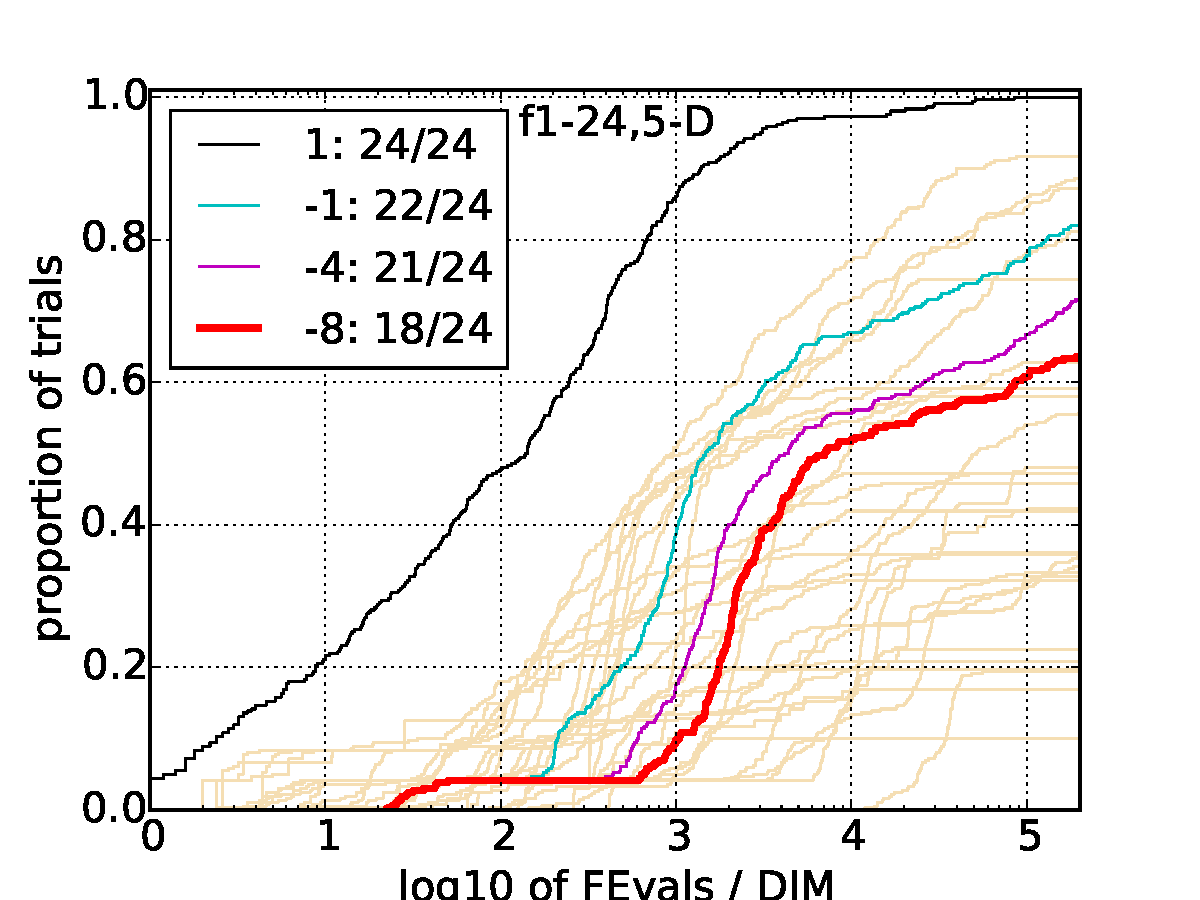
\includegraphics[width=0.528\textwidth,trim=0 0mm 16mm 11mm, clip]{pprldistr_05D_noiselessall} &
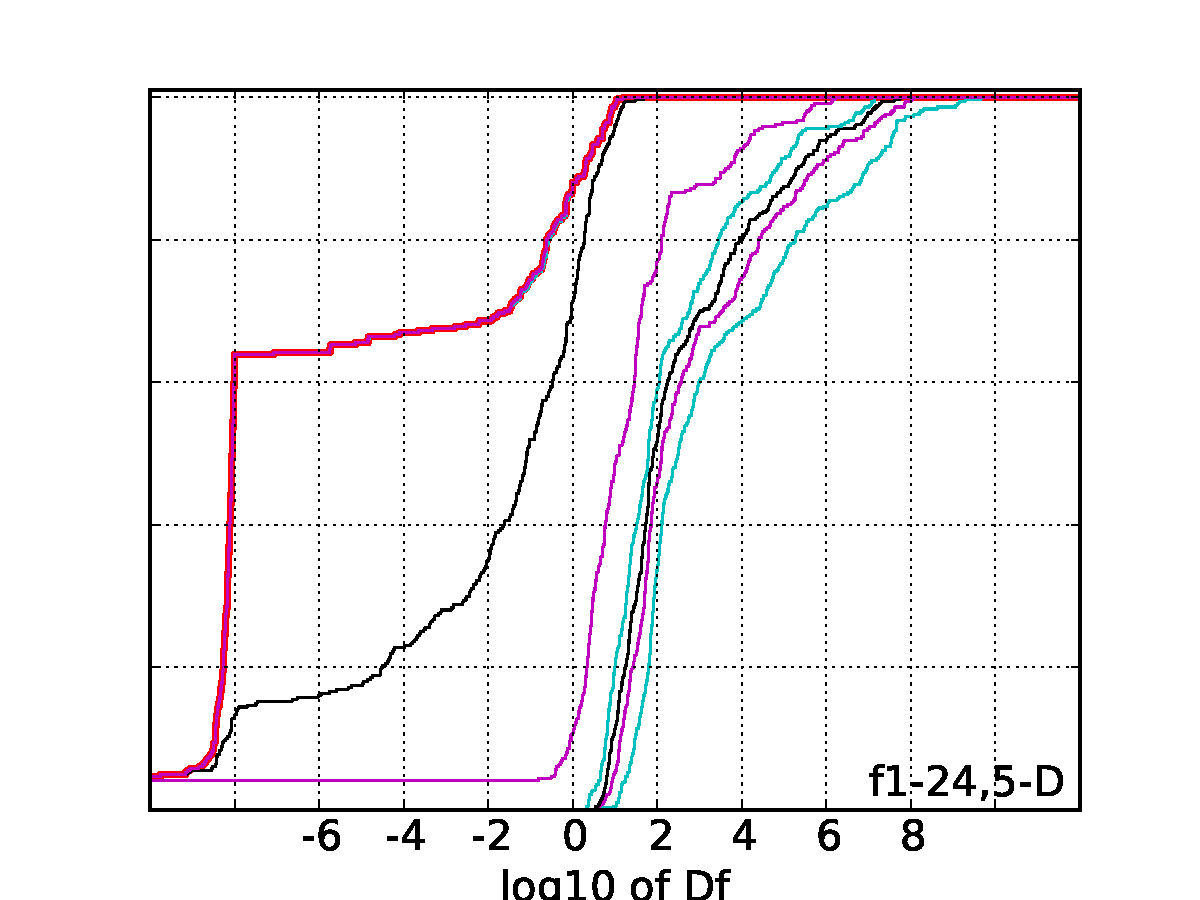
\includegraphics[width=0.46\textwidth,trim=24mm 0mm 16mm 11mm, clip]{ppfvdistr_05D_noiselessall}\\
\rot[5]{all functions}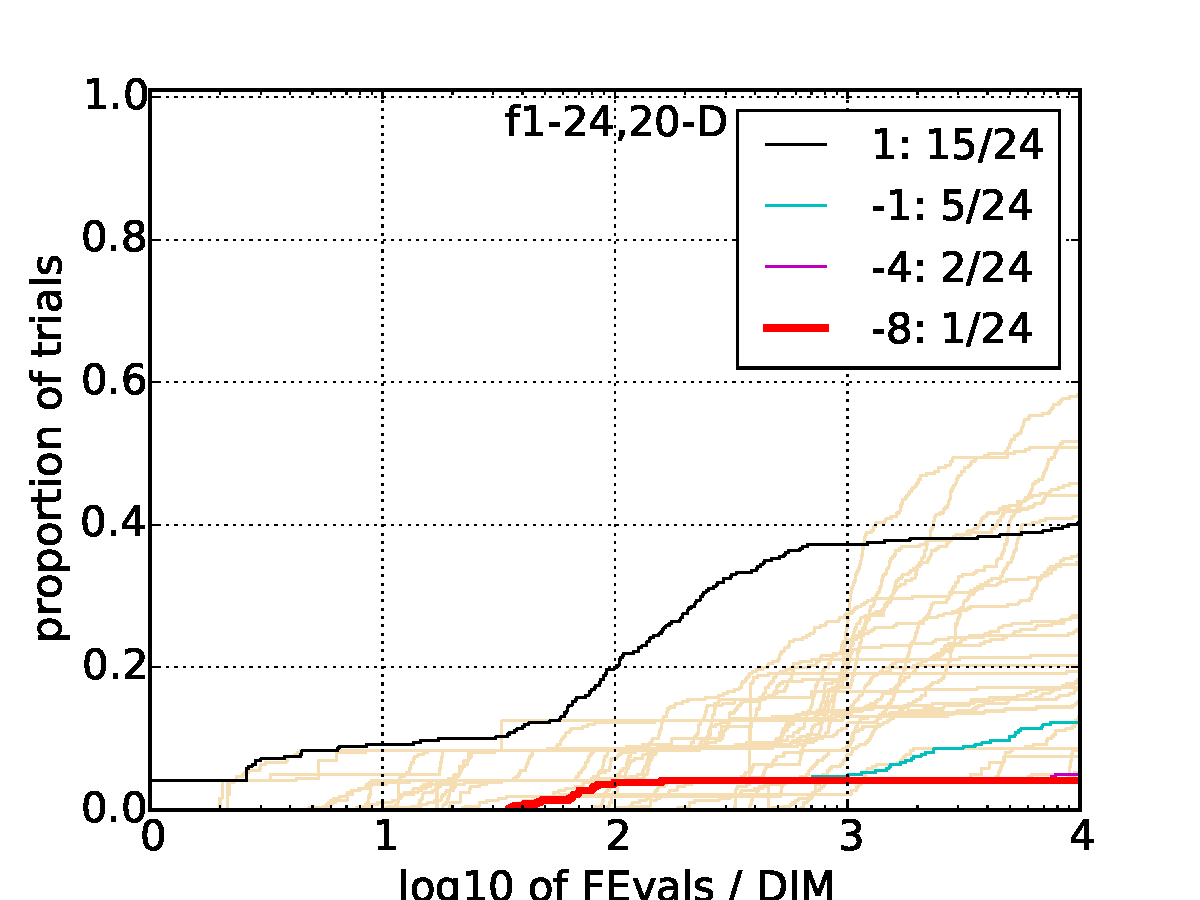
\includegraphics[width=0.528\textwidth,trim=0 0mm 16mm 11mm, clip]{pprldistr_20D_noiselessall} &
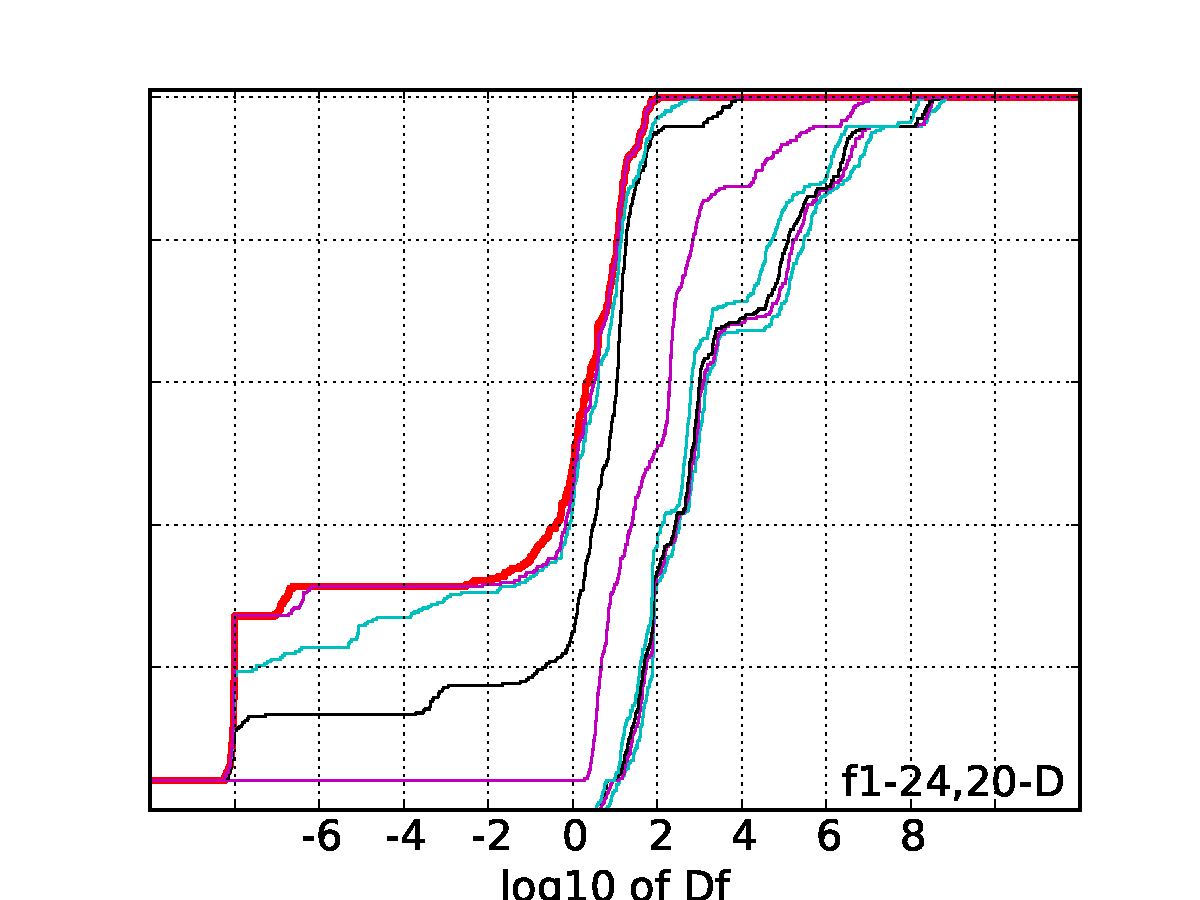
\includegraphics[width=0.46\textwidth,trim=24mm 0mm 16mm 11mm, clip]{ppfvdistr_20D_noiselessall}
\end{tabular}
\caption{\label{fig:RLDs05Da\algfolder} \bbobpprldistrlegend{} The top row shows results for 5-D and the bottom row for 20-D.}
\end{figure}
%%%%%%%%%%%%%%%%%%%%%%%%%%%%%%%%%%%%%%%%%%%%%%%%%%%%%%%%%%%%%%%%%%%%%%%%%%%%%%%
%%%%%%%%%%%%%%%%%%%%%%%%%%%%%%%%%%%%%%%%%%%%%%%%%%%%%%%%%%%%%%%%%%%%%%%%%%%%%%%
\begin{figure}[htbp!]
\centering
\begin{tabular}{@{}c@{}c@{}}
\rot[2.5]{separable fcts}
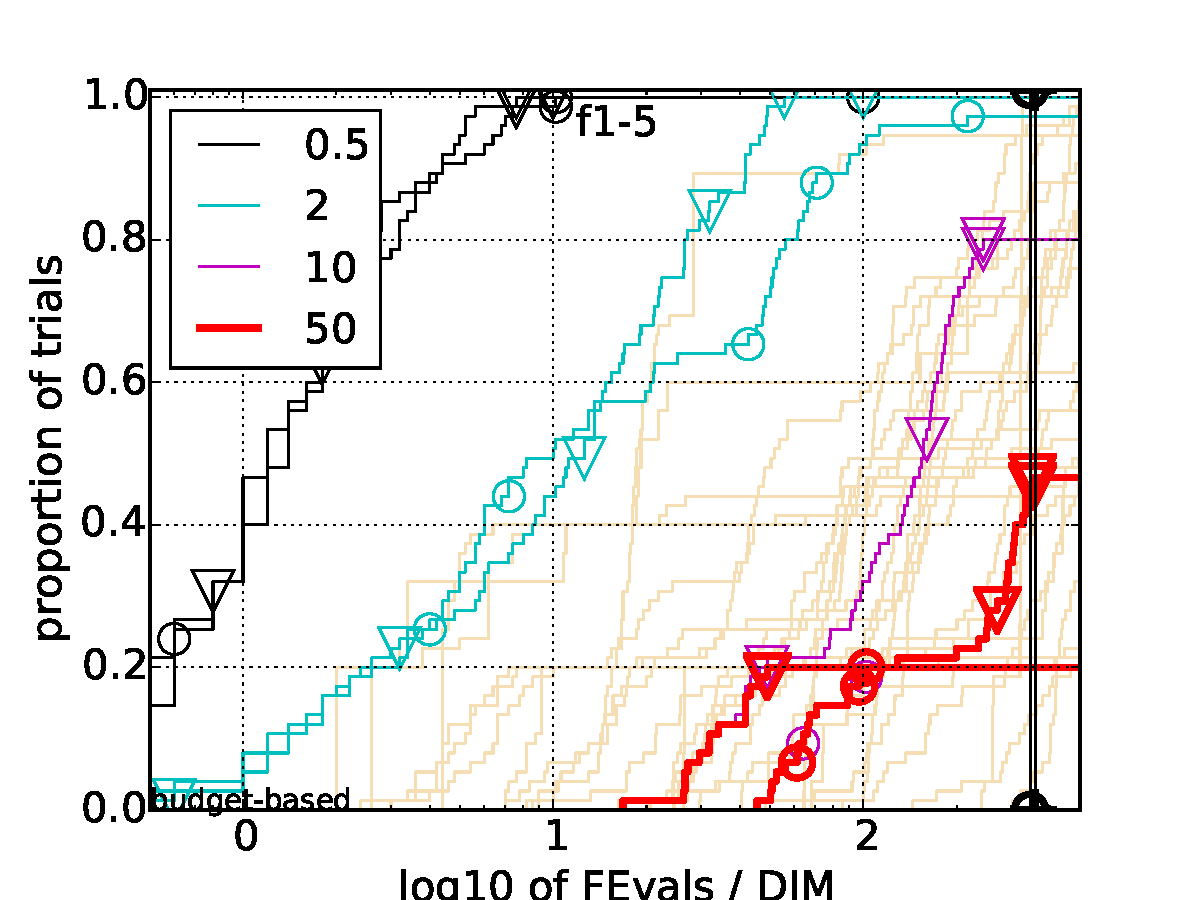
\includegraphics[width=0.41\textwidth,trim=0 7.5mm 16mm 11mm, clip]{pprldistr_05D_separ} &
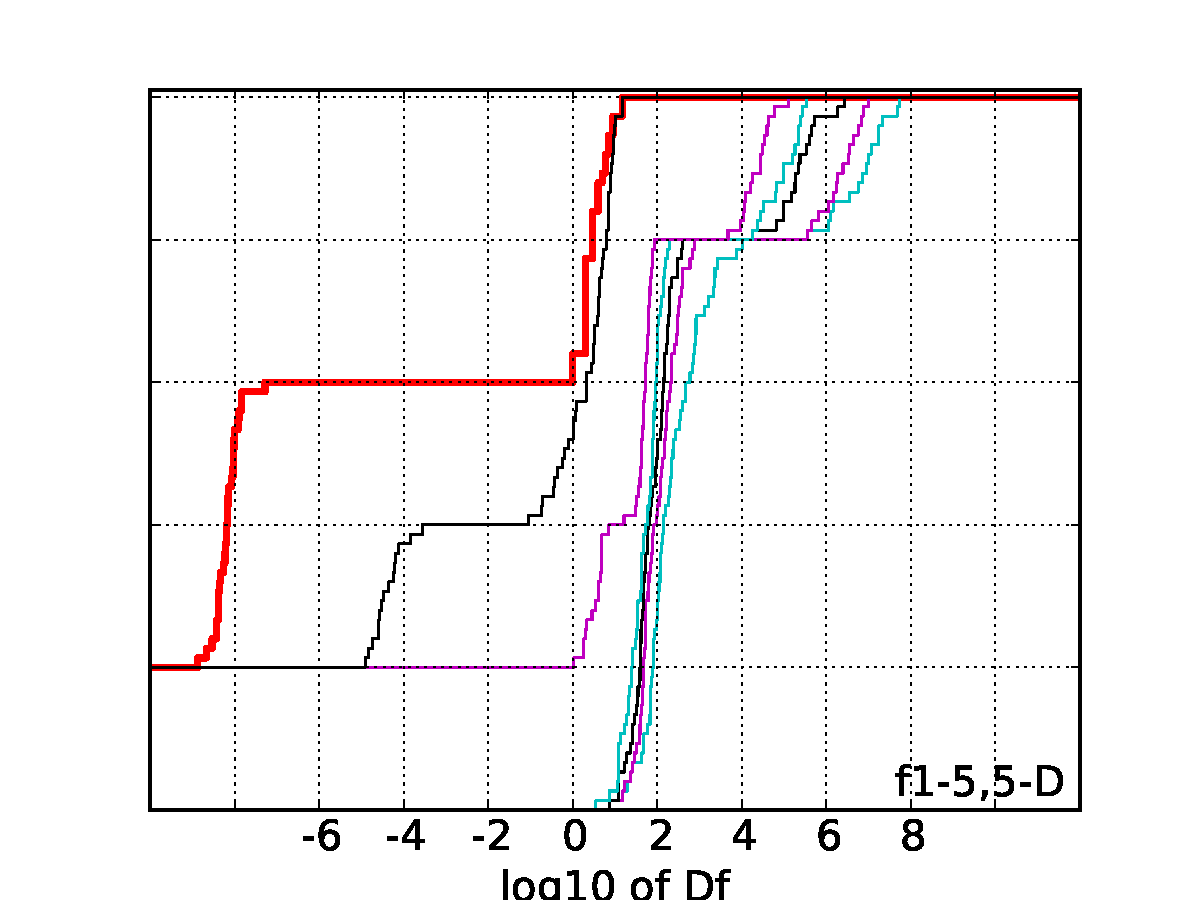
\includegraphics[width=0.3579\textwidth,trim=24mm 7.5mm 16mm 11mm, clip]{ppfvdistr_05D_separ}
\\[-1ex]
\rot[1.3]{misc.\ moderate fcts}
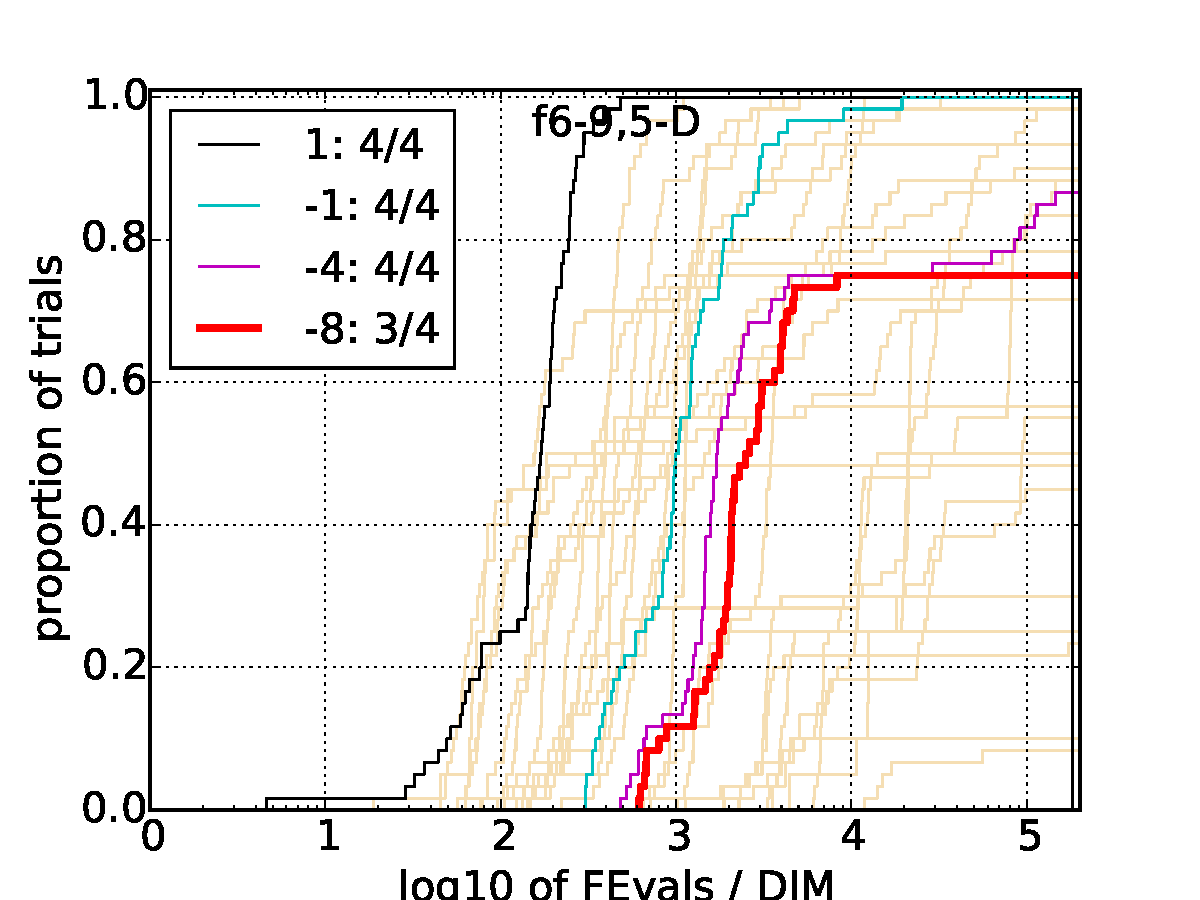
\includegraphics[width=0.41\textwidth,trim=0 7.5mm 16mm 11mm, clip]{pprldistr_05D_lcond} &
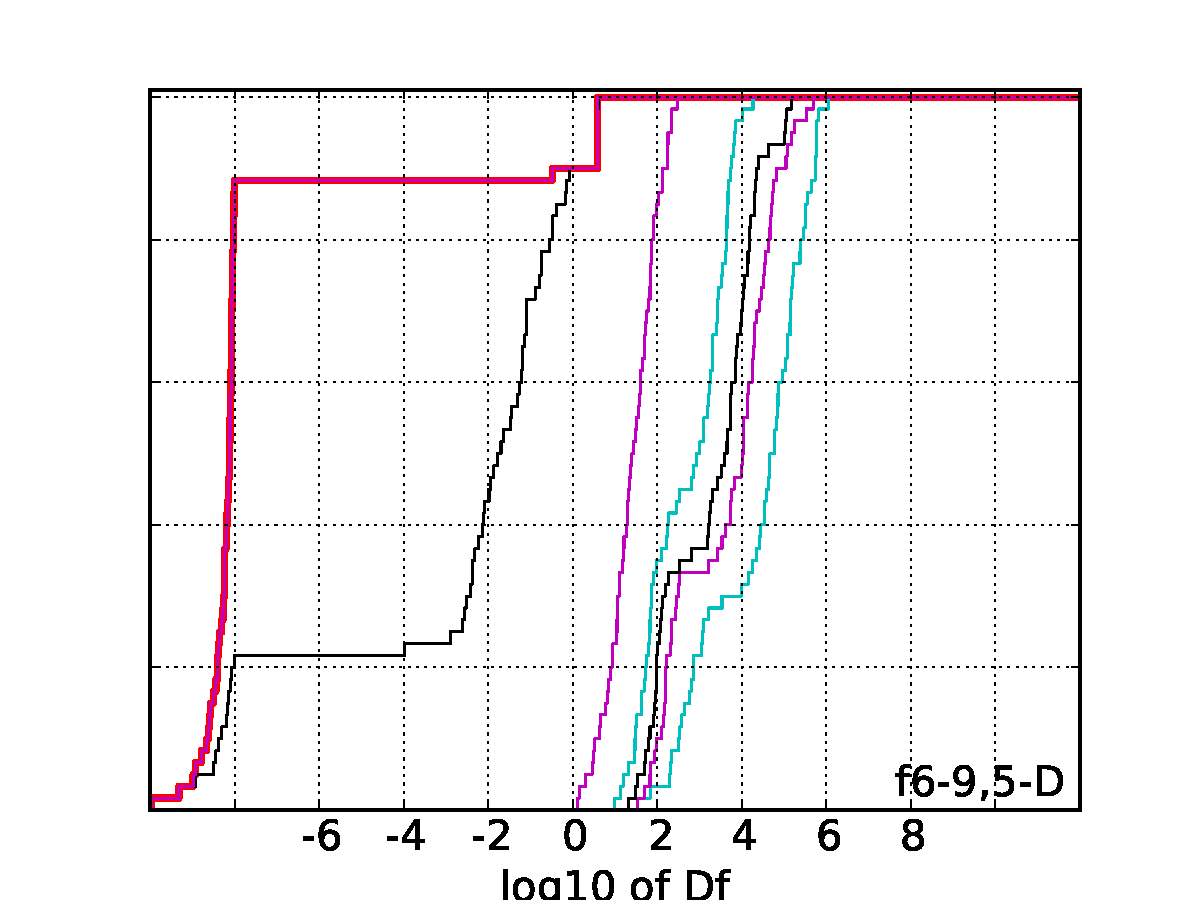
\includegraphics[width=0.3579\textwidth,trim=24mm 7.5mm 16mm 11mm, clip]{ppfvdistr_05D_lcond}
\\[-1ex]
\rot[1.1]{ill-conditioned fcts}
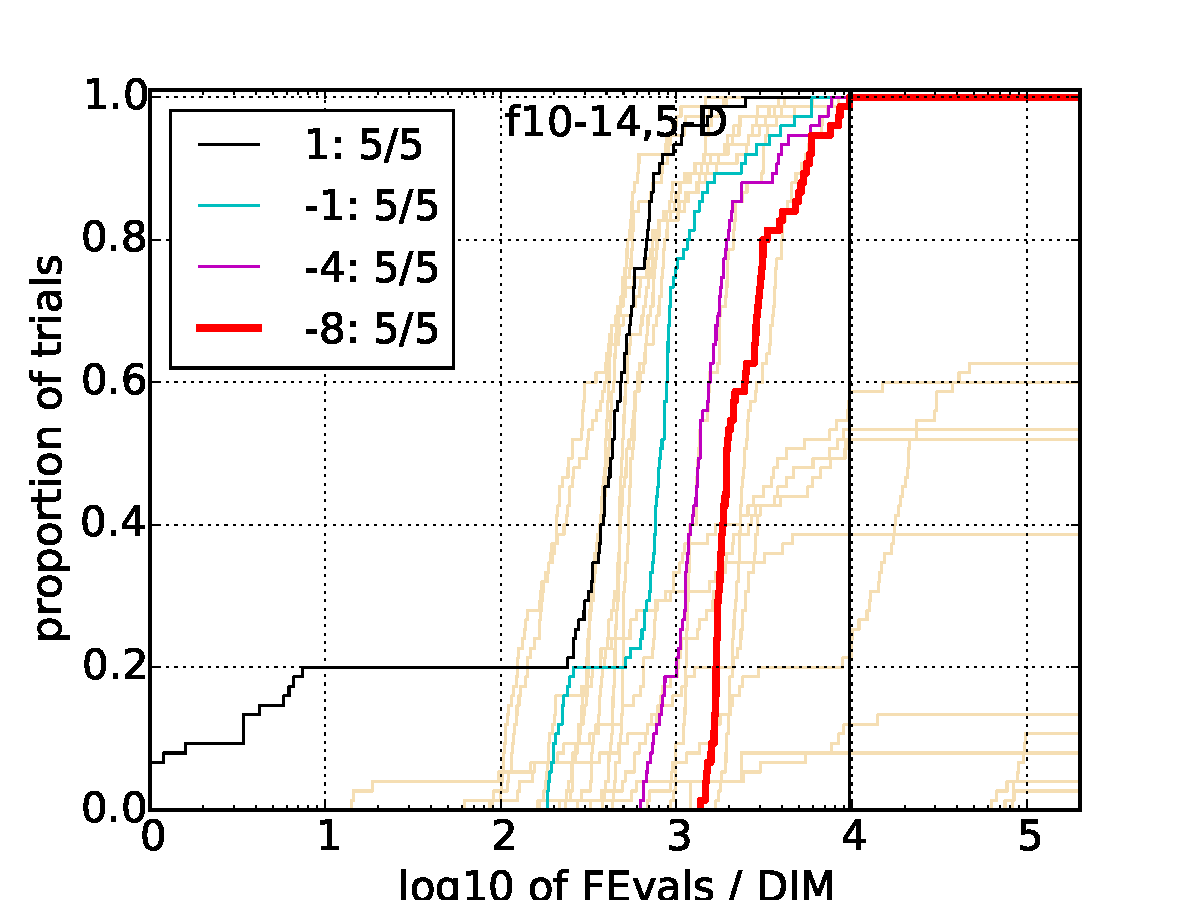
\includegraphics[width=0.41\textwidth,trim=0 7.5mm 16mm 11mm, clip]{pprldistr_05D_hcond} &
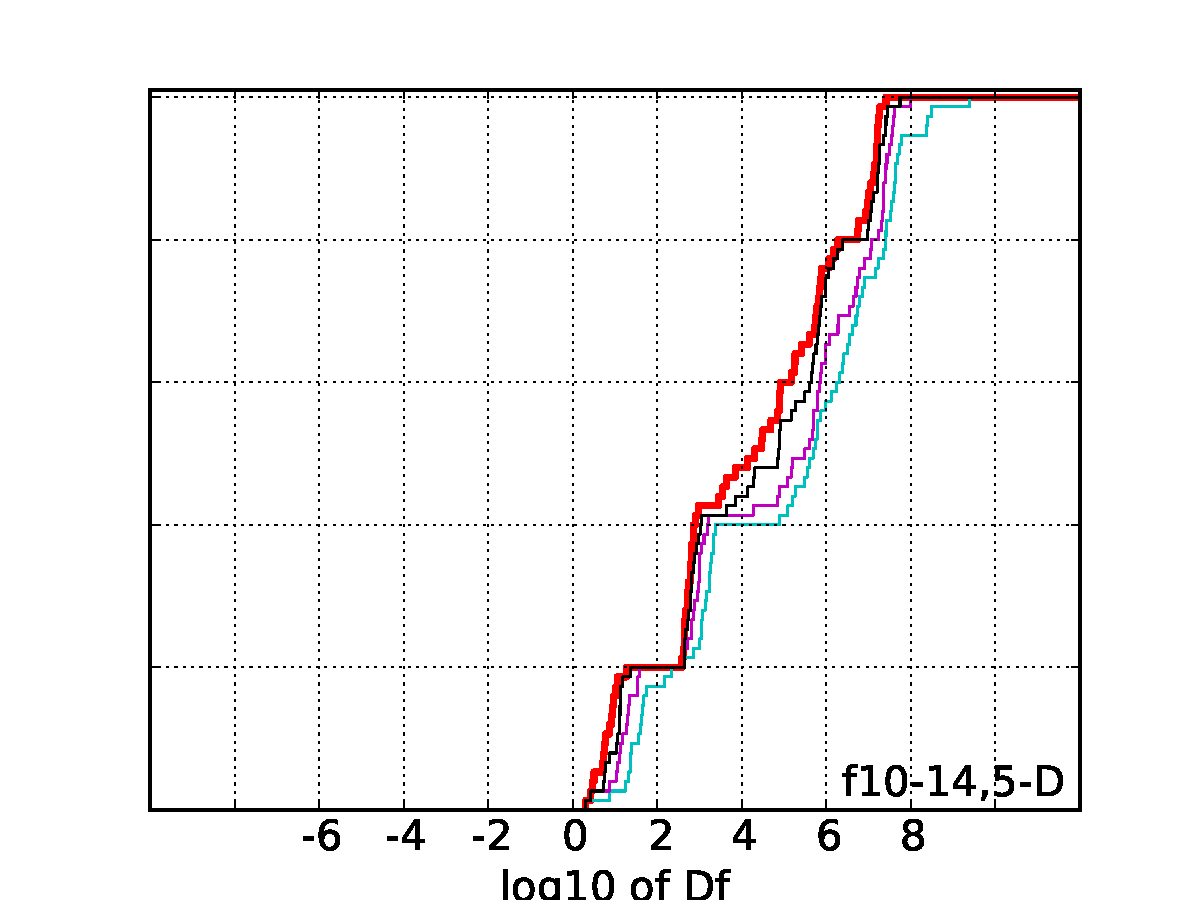
\includegraphics[width=0.3579\textwidth,trim=24mm 7.5mm 16mm 11mm, clip]{ppfvdistr_05D_hcond}
\\[-1ex]
\rot[1.7]{multi-modal fcts}
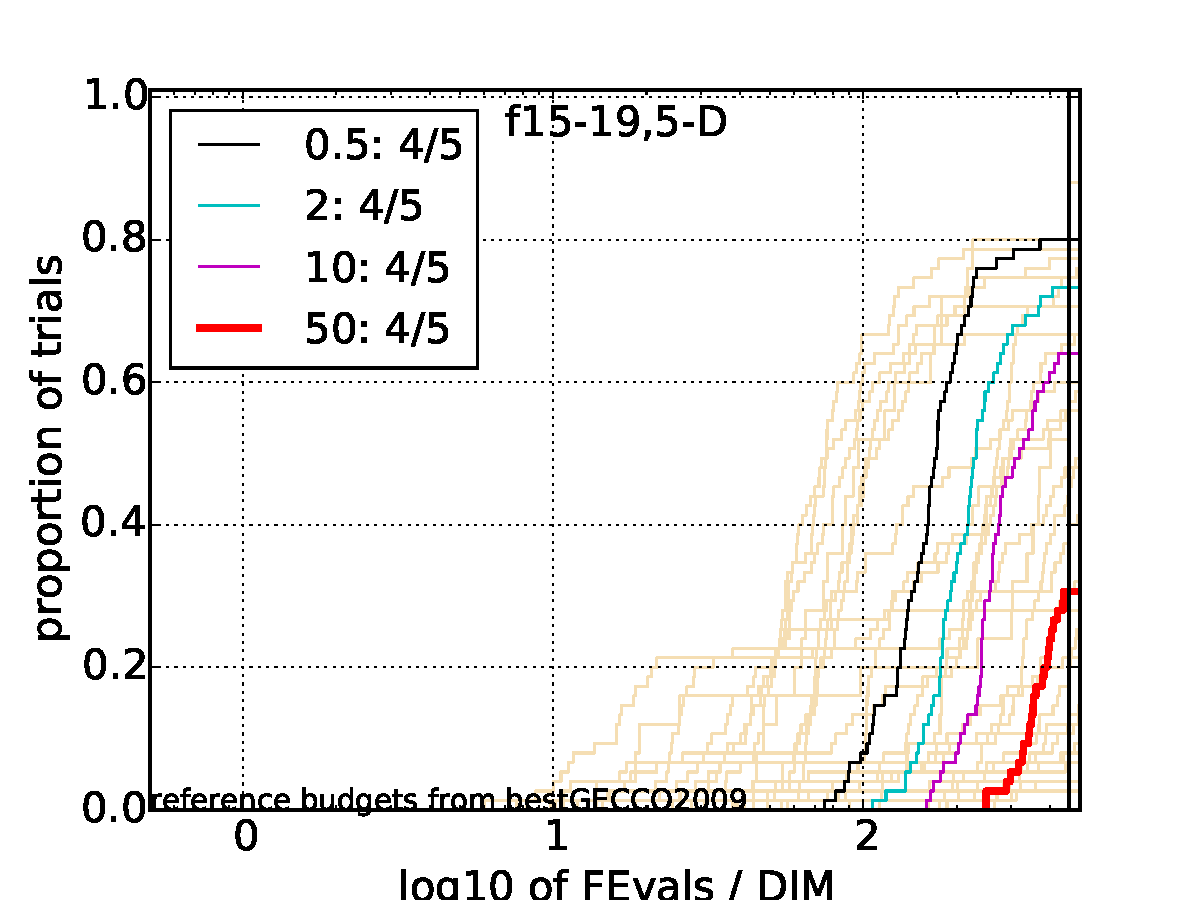
\includegraphics[width=0.41\textwidth,trim=0 7.5mm 16mm 11mm, clip]{pprldistr_05D_multi} &
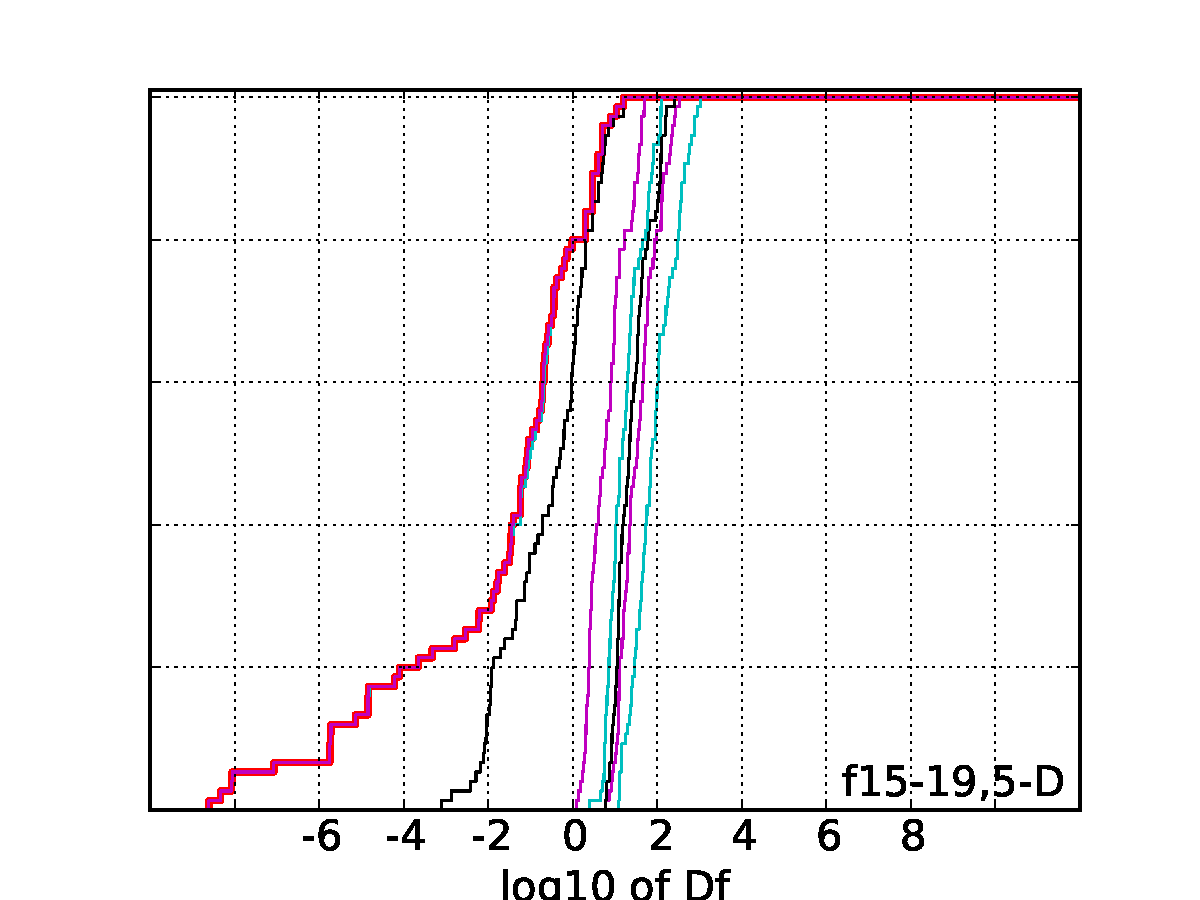
\includegraphics[width=0.3579\textwidth,trim=24mm 7.5mm 16mm 11mm, clip]{ppfvdistr_05D_multi}
\\[-1ex]
\rot[1.5]{weak structure fcts}
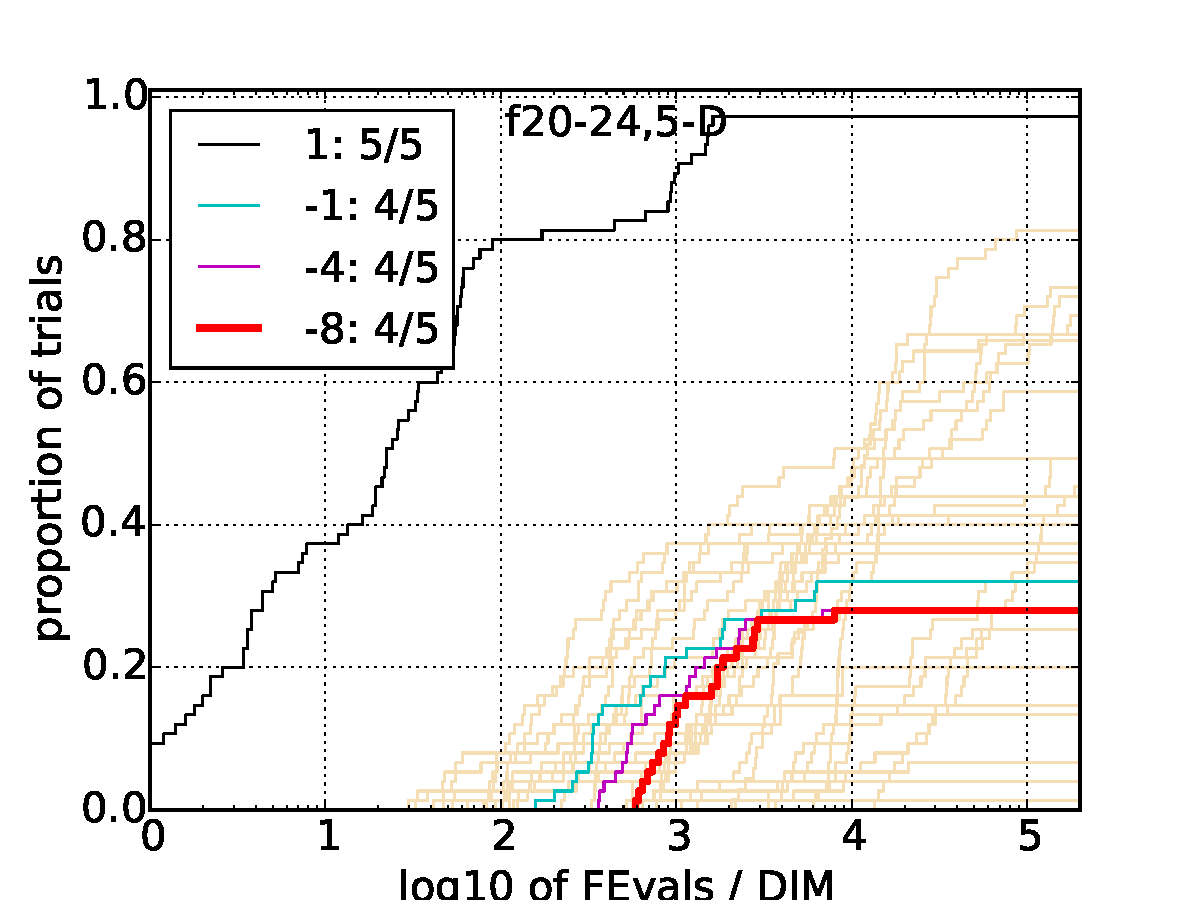
\includegraphics[width=0.41\textwidth,trim=0 0mm 16mm 11mm, clip]{pprldistr_05D_mult2} &
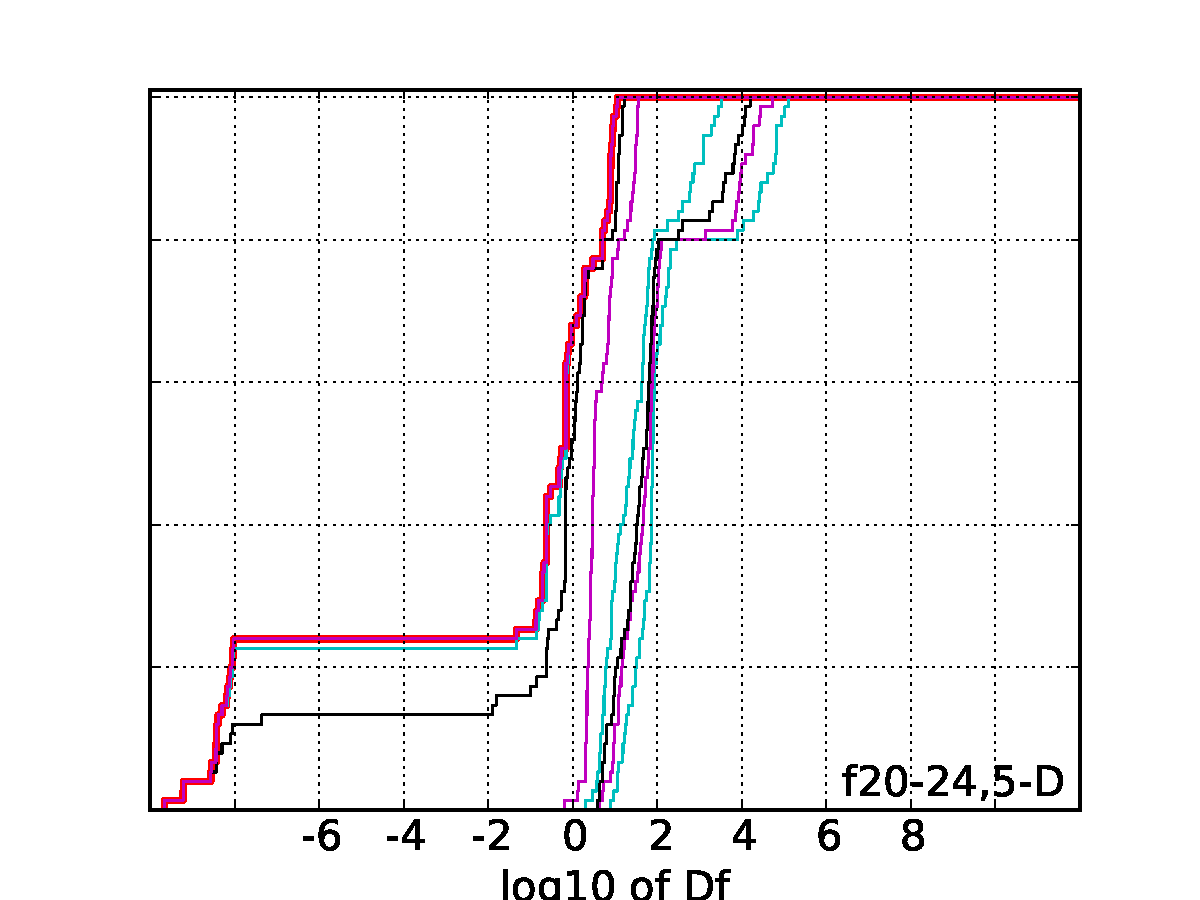
\includegraphics[width=0.3579\textwidth,trim=24mm 0mm 16mm 11mm, clip]{ppfvdistr_05D_mult2}
\end{tabular}
\vspace*{-0.5ex}
\caption{\label{fig:RLDs05Db\algfolder}Subgroups of functions 5-D. See caption of Figure~\ref{fig:RLDs05Da\algfolder} for details.
%Left subplots: Empirical Cumulative Distribution Function (ECDF) of the running time (number of function evaluations),
%divided by search space dimension $D$, to fall below $\fopt+\Df$ with
%$\Df=10^{k}$, where $k$ is the first value in the legend. The vertical black
%line indicates the maximum number of function evaluations. The legends indicate
%the number of functions that were solved in at least one trial.
%% FEvals denotes number of function evaluations,
%Light brown lines in the background show ECDFs for target value $10^{-8}$ of
%all algorithms benchmarked during BBOB 2009. Right subplots: ECDF of
%the best achieved \Df\ divided by $10^k$ (upper left lines in continuation of
%the left subplot), and best achieved \Df\ divided by $10^{-8}$ for running
%times of $D, 10\,D, 100\,D\dots$ function evaluations (from right to left
%cycling black-cyan-magenta).
%%Top row: all functions; second row: separable
%%functions; third row: misc.\ moderate functions; fourth row:
%%ill-conditioned functions; fifth row: multi-modal functions with
%%adequate structure; last row: multi-modal functions with weak structure.
%$D=\mathsf{DIM}$ denotes search space dimension (5 in this case) and $\Df=\mathsf{Df}$
%denotes the difference to the optimal function value.
}
\end{figure}
%%%%%%%%%%%%%%%%%%%%%%%%%%%%%%%%%%%%%%%%%%%%%%%%%%%%%%%%%%%%%%%%%%%%%%%%%%%%%%%
%%%%%%%%%%%%%%%%%%%%%%%%%%%%%%%%%%%%%%%%%%%%%%%%%%%%%%%%%%%%%%%%%%%%%%%%%%%%%%%
\begin{figure}[htbp!]
\centering
\begin{tabular}{@{}c@{}c@{}}
\rot[2.5]{separable fcts}
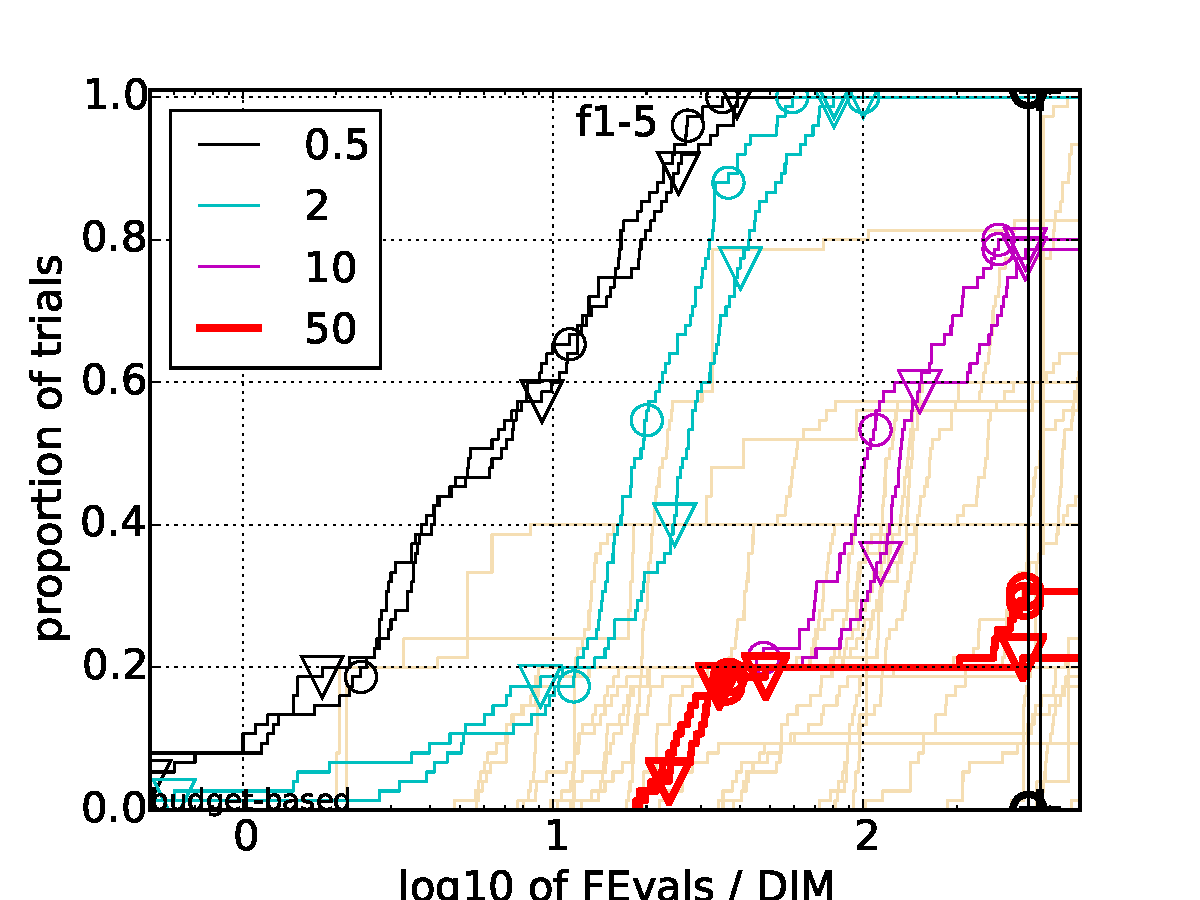
\includegraphics[width=0.41\textwidth,trim=0 7.5mm 16mm 11mm, clip]{pprldistr_20D_separ} &
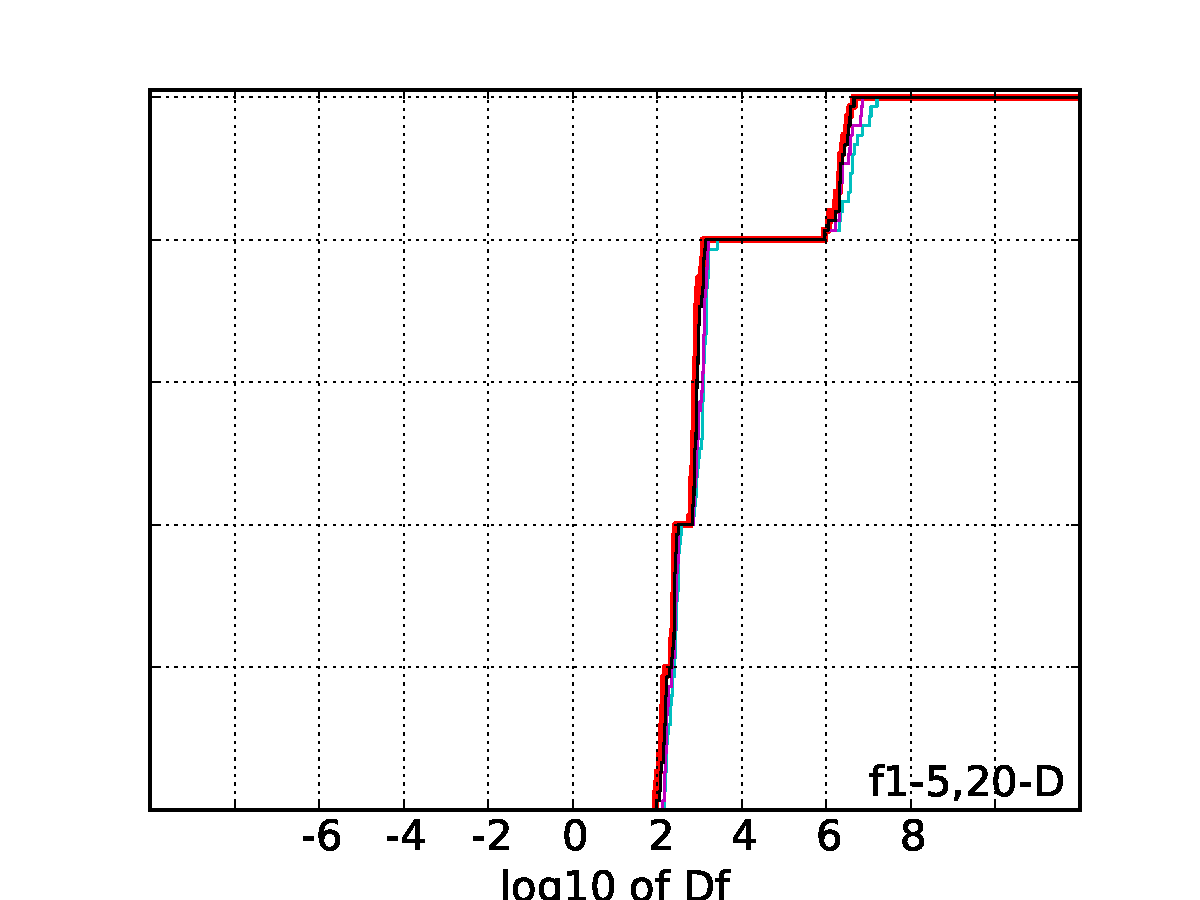
\includegraphics[width=0.3579\textwidth,trim=24mm 7.5mm 16mm 11mm, clip]{ppfvdistr_20D_separ}
\\[-1ex]
\rot[1.3]{misc.\ moderate fcts}
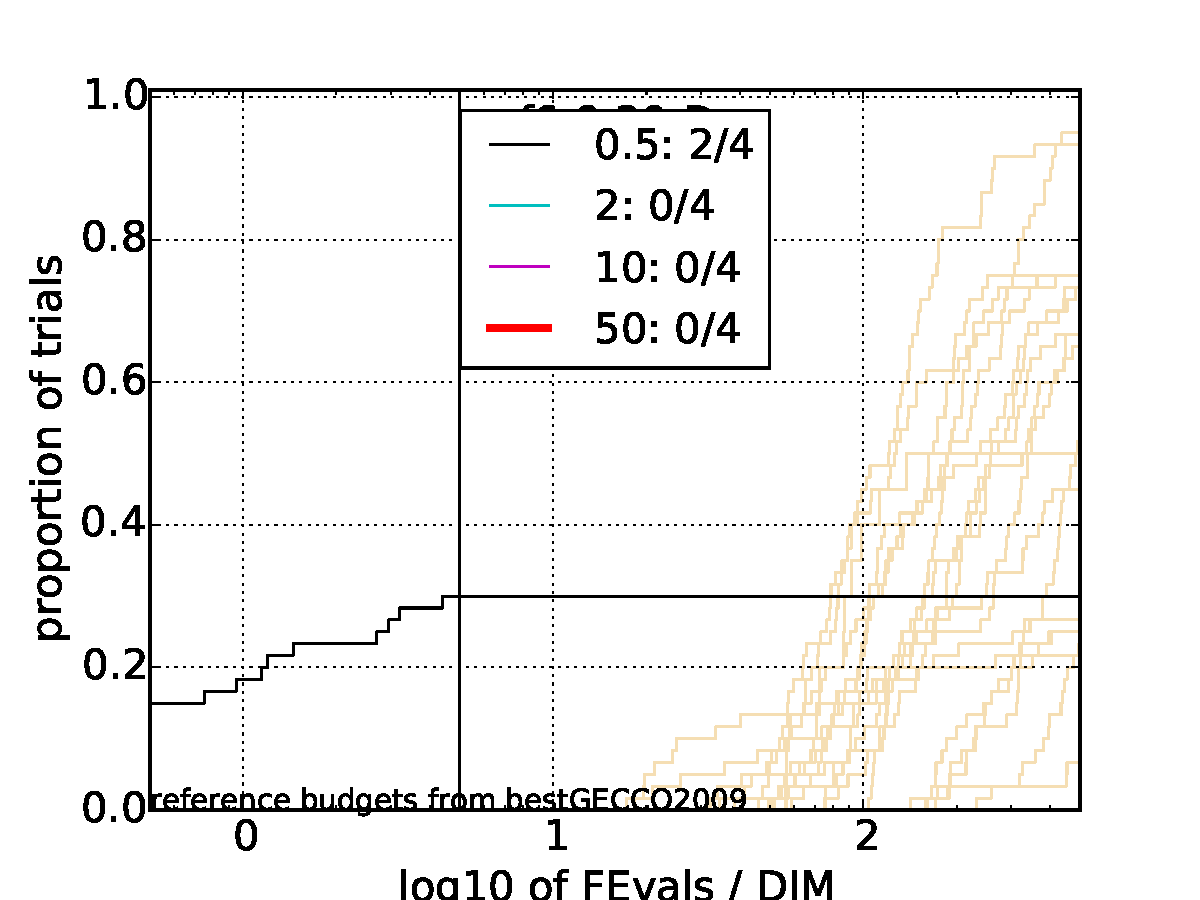
\includegraphics[width=0.41\textwidth,trim=0 7.5mm 16mm 11mm, clip]{pprldistr_20D_lcond} &
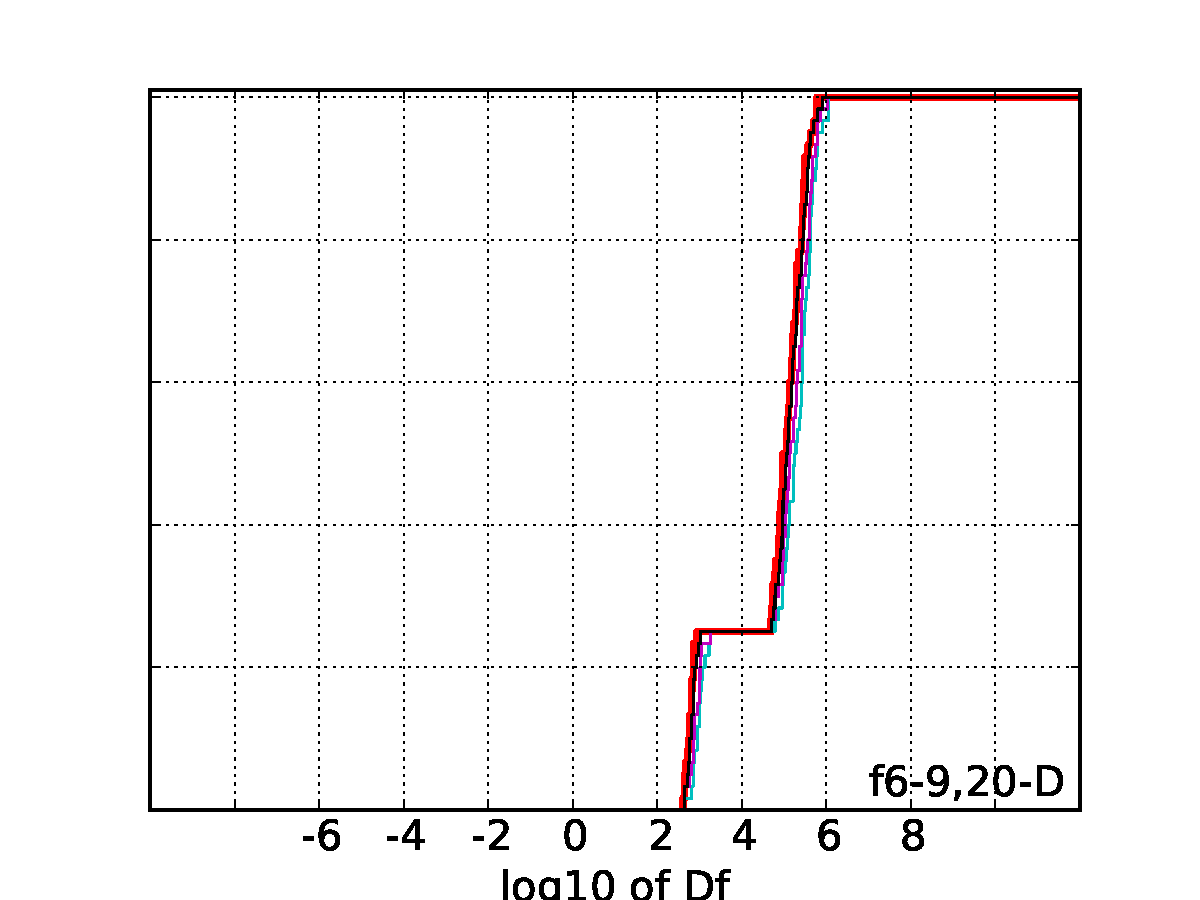
\includegraphics[width=0.3579\textwidth,trim=24mm 7.5mm 16mm 11mm, clip]{ppfvdistr_20D_lcond}
\\[-1ex]
\rot[1.1]{ill-conditioned fcts}
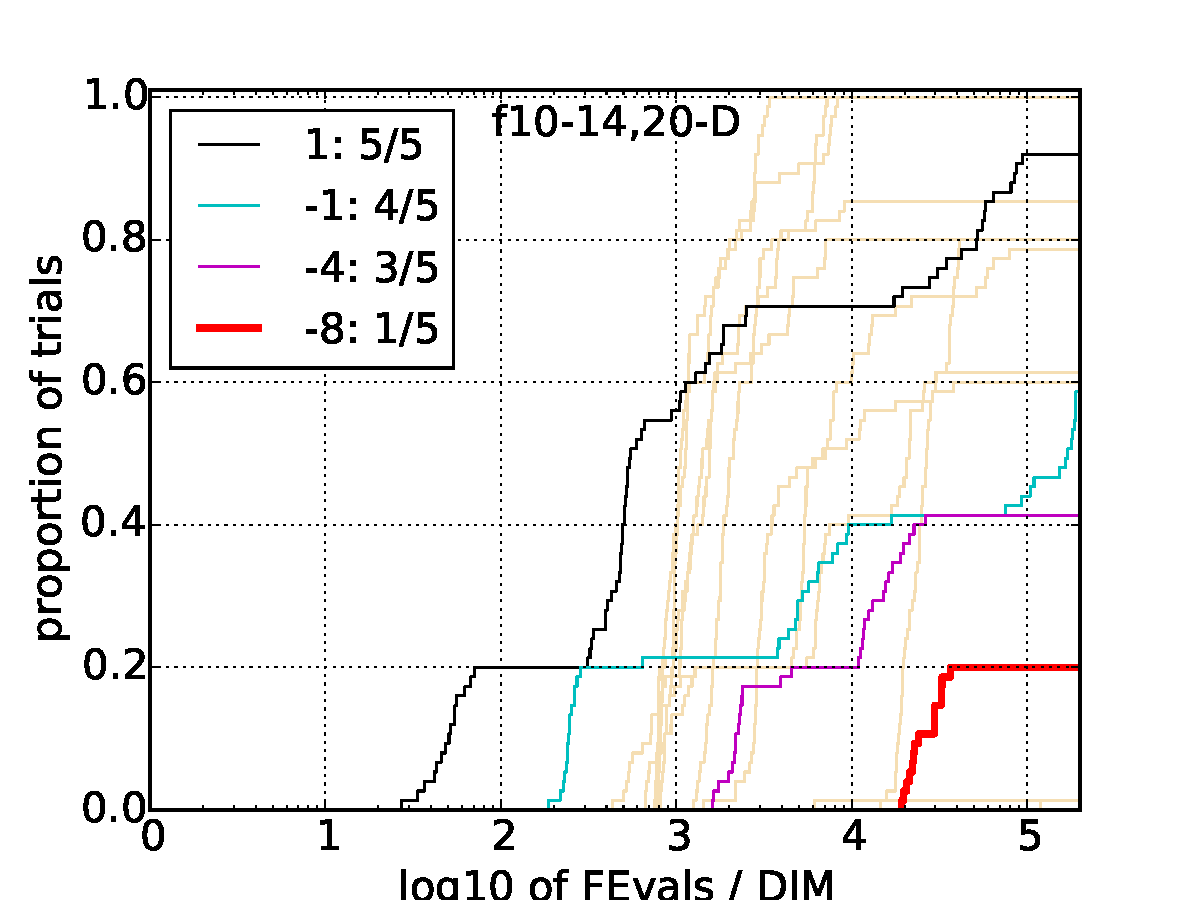
\includegraphics[width=0.41\textwidth,trim=0 7.5mm 16mm 11mm, clip]{pprldistr_20D_hcond} &
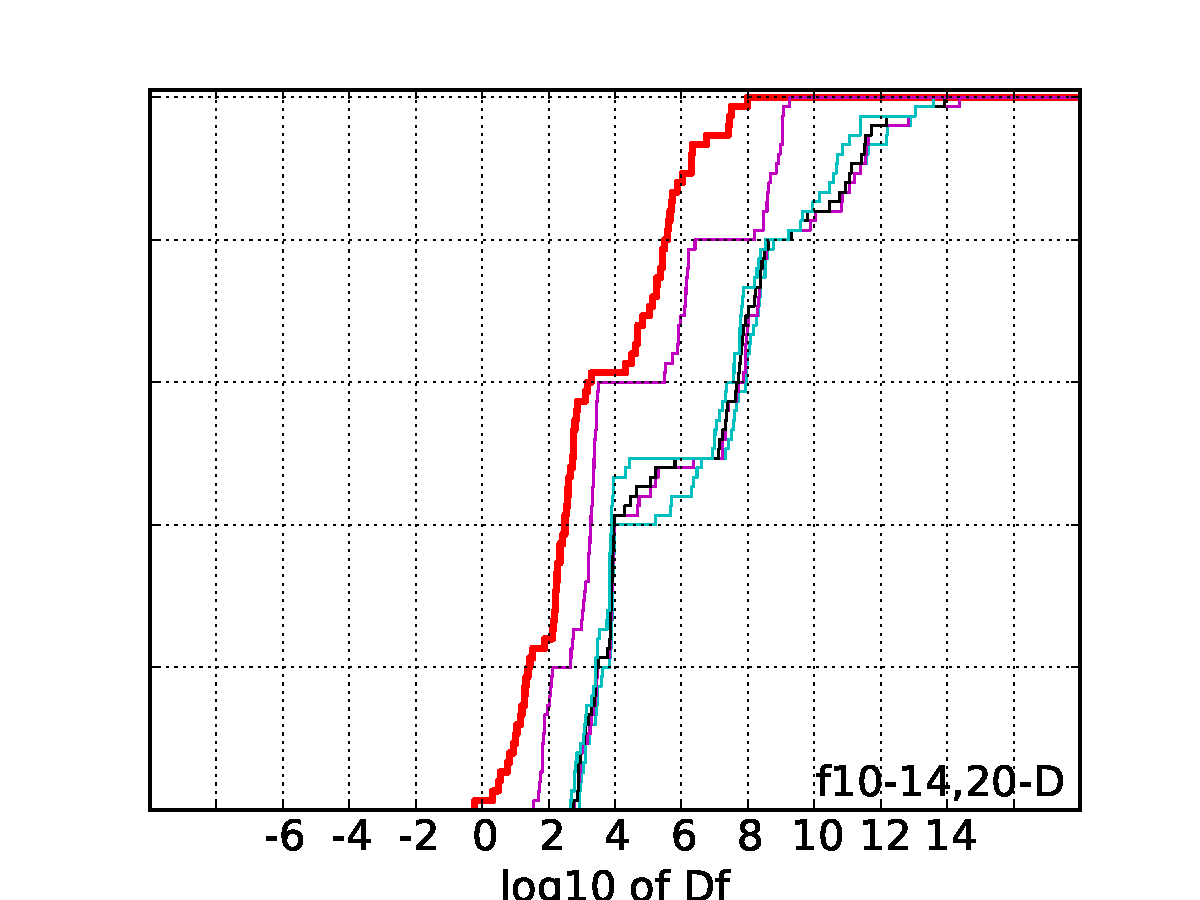
\includegraphics[width=0.3579\textwidth,trim=24mm 7.5mm 16mm 11mm, clip]{ppfvdistr_20D_hcond}
\\[-1ex]
\rot[1.7]{multi-modal fcts}
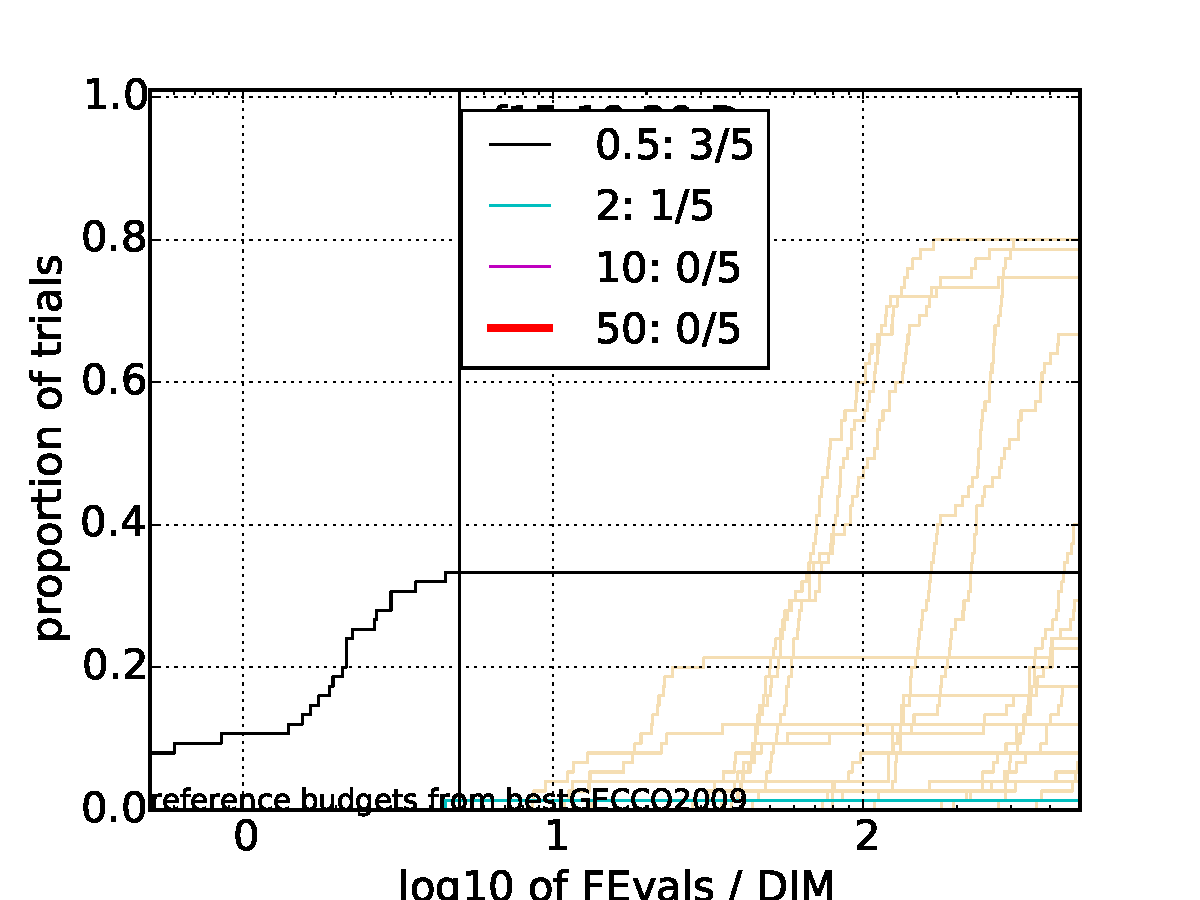
\includegraphics[width=0.41\textwidth,trim=0 7.5mm 16mm 11mm, clip]{pprldistr_20D_multi} &
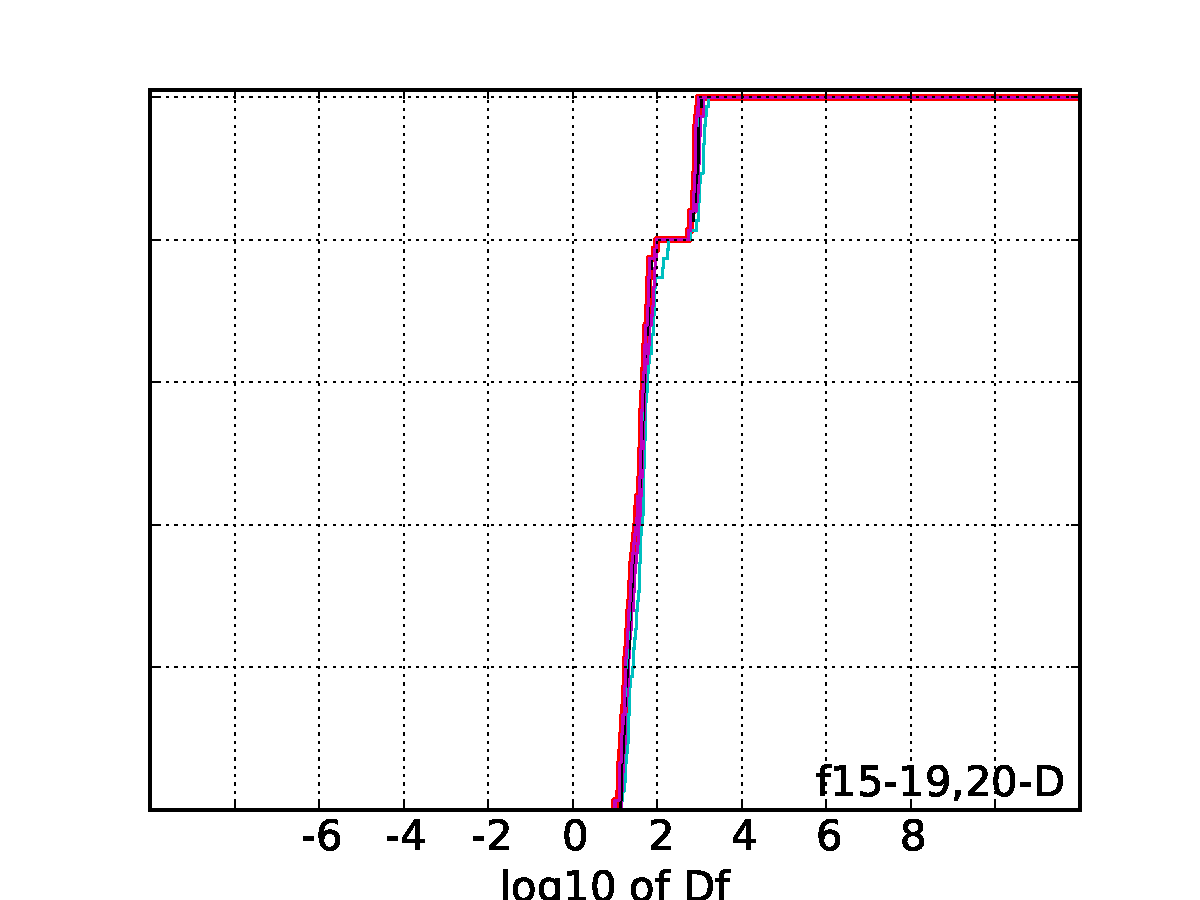
\includegraphics[width=0.3579\textwidth,trim=24mm 7.5mm 16mm 11mm, clip]{ppfvdistr_20D_multi}
\\[-1ex]
\rot[1.5]{weak structure fcts}
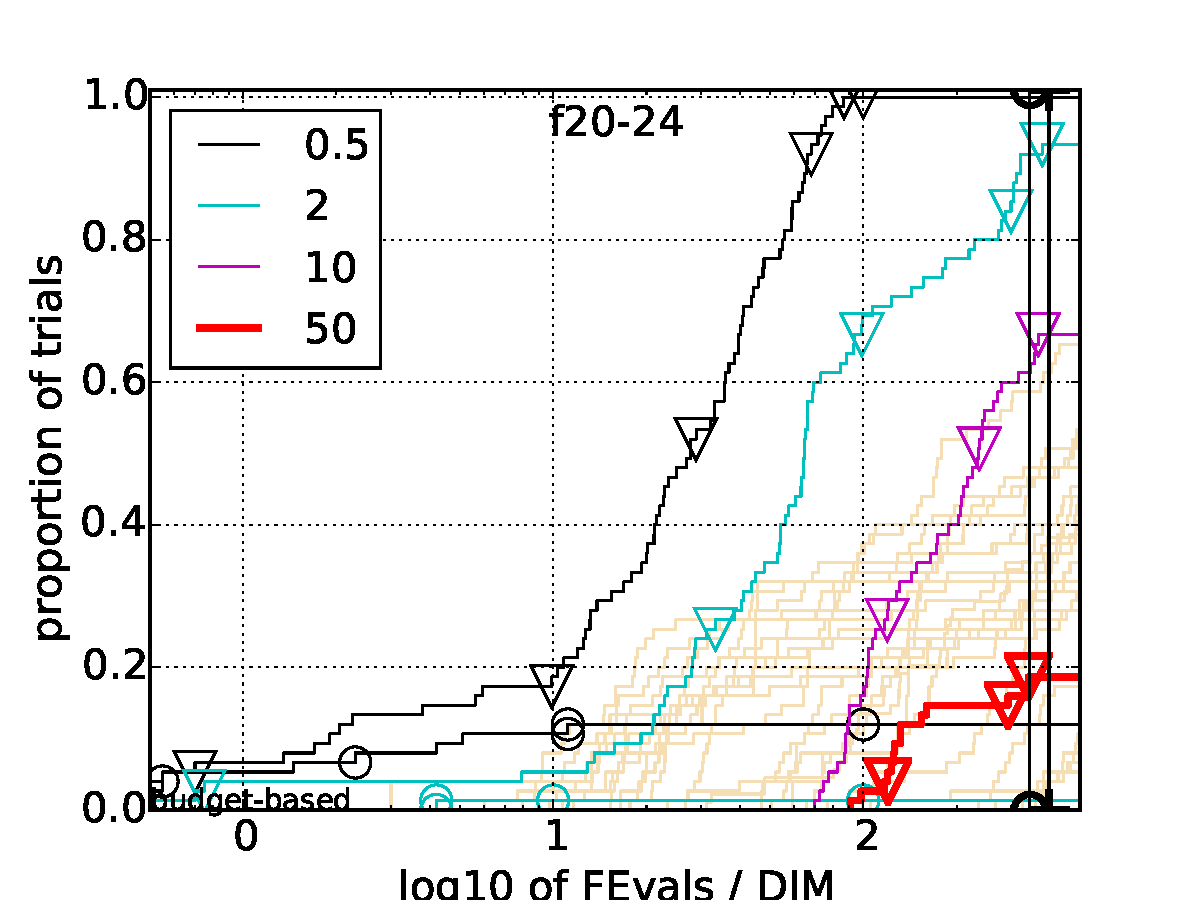
\includegraphics[width=0.41\textwidth,trim=0 0mm 16mm 11mm, clip]{pprldistr_20D_mult2} &
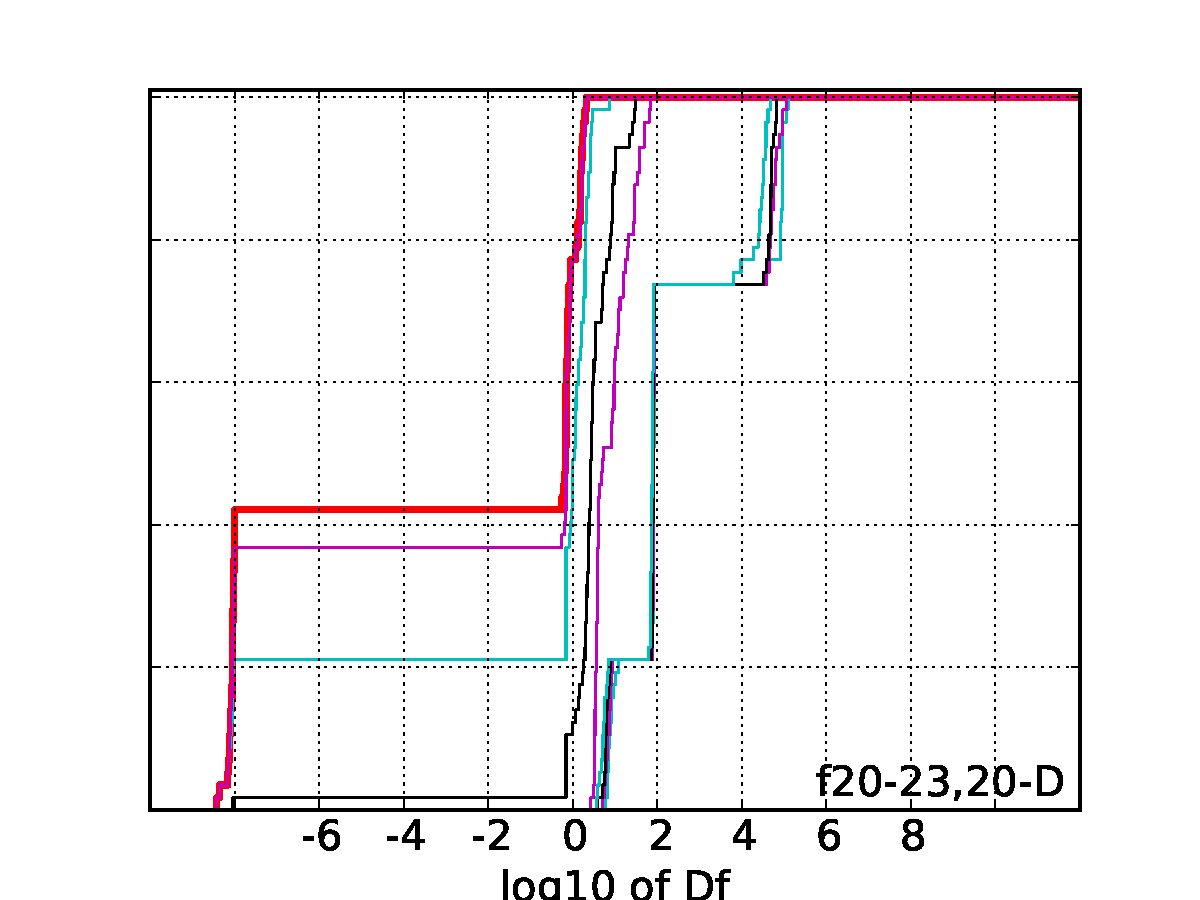
\includegraphics[width=0.3579\textwidth,trim=24mm 0mm 16mm 11mm, clip]{ppfvdistr_20D_mult2}
\end{tabular}
\vspace*{-0.5ex}
\caption{\label{fig:RLDs20Db\algfolder}Subgroups of functions 20-D. See caption
of Figure~\ref{fig:RLDs05Da\algfolder} for details.}
\end{figure}
%%%%%%%%%%%%%%%%%%%%%%%%%%%%%%%%%%%%%%%%%%%%%%%%%%%%%%%%%%%%%%%%%%%%%%%%%%%%%%%
%%%%%%%%%%%%%%%%%%%%%%%%%%%%%%%%%%%%%%%%%%%%%%%%%%%%%%%%%%%%%%%%%%%%%%%%%%%%%%%
\begin{figure}[htbp!]
\subfloat{
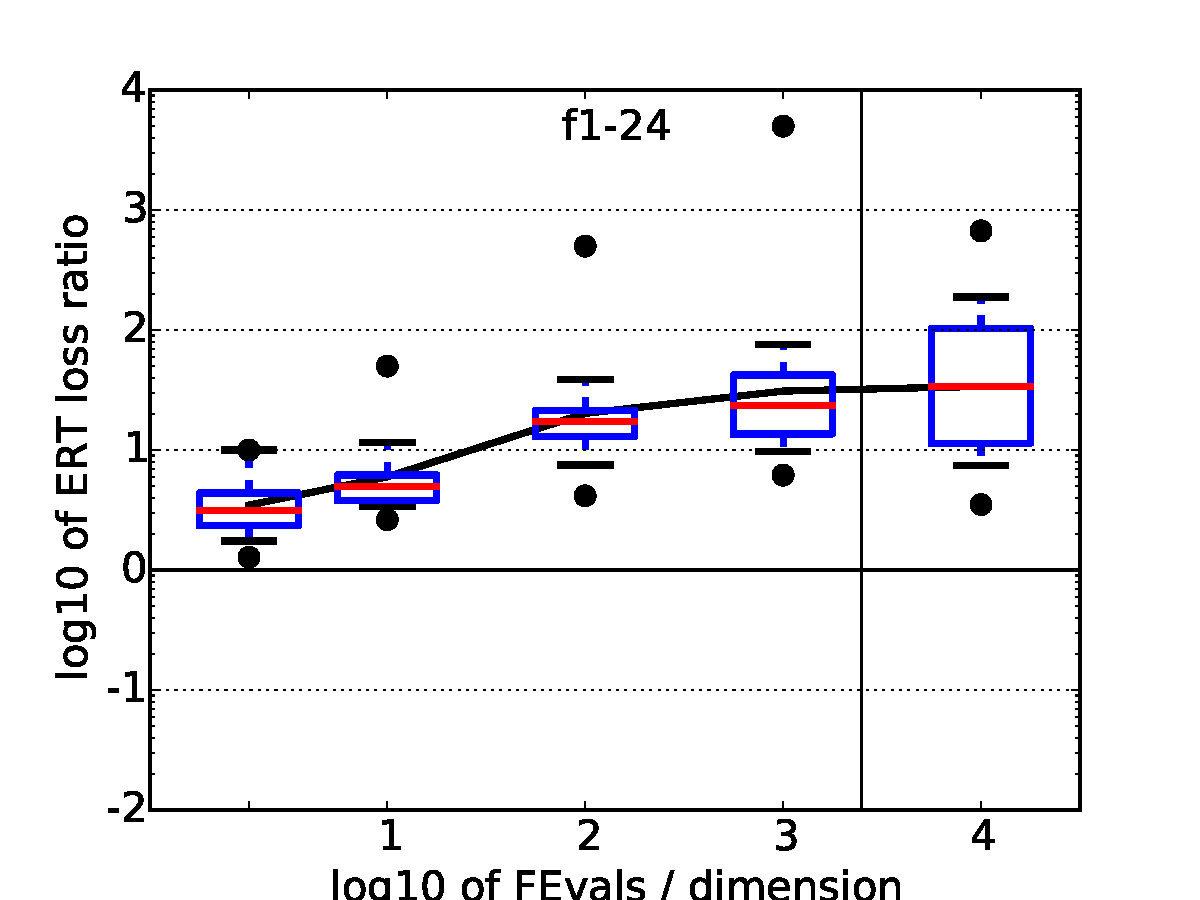
\includegraphics[width=0.35\textwidth,trim=9mm 8mm 18mm 12mm, clip]{pplogloss_05D_noiselessall}
}
\subfloat{
\centering
\scriptsize
\input{\bbobdatapath\algfolder pploglosstable_05D_noiselessall}}\\[-2ex]
\subfloat{
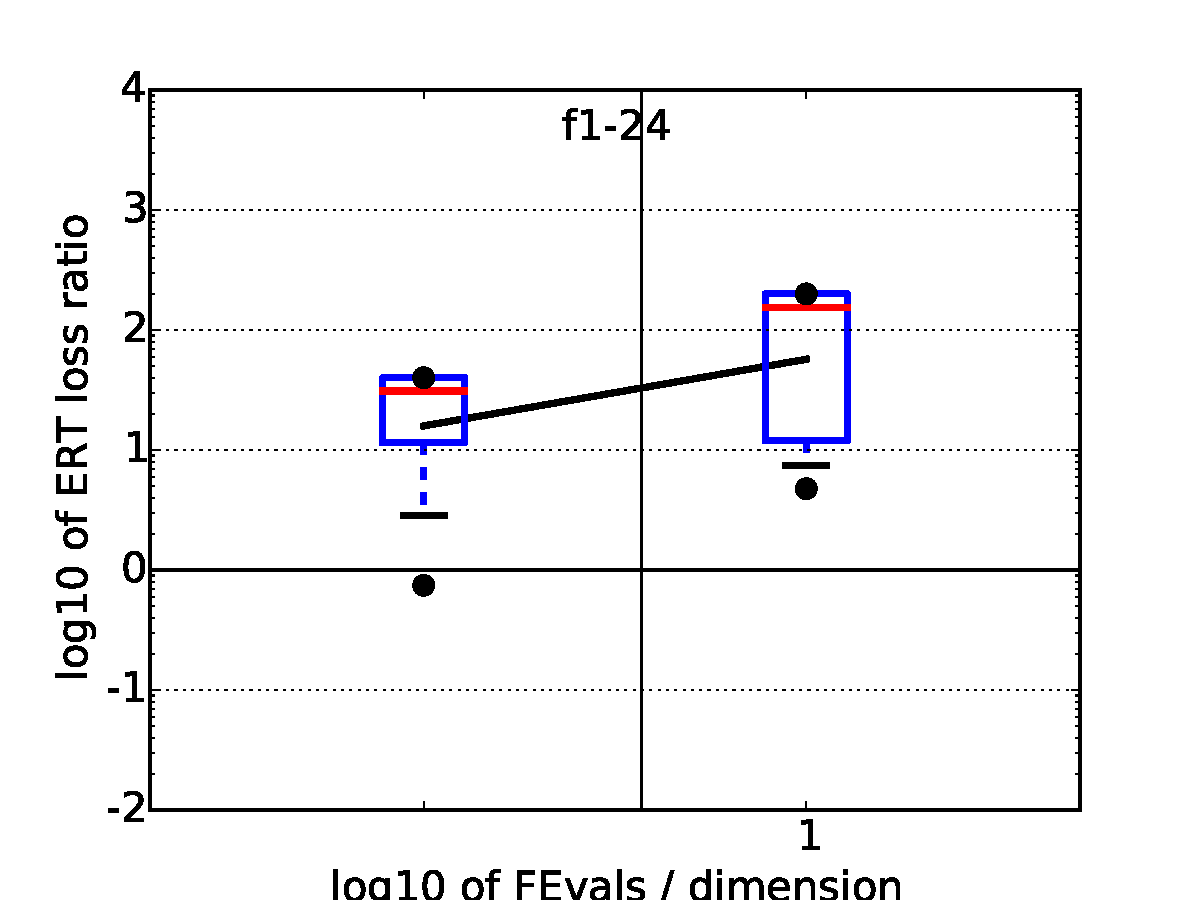
\includegraphics[width=0.35\textwidth,trim=9mm 0mm 18mm 12mm, clip]{pplogloss_20D_noiselessall}
}
\subfloat{
\centering
\scriptsize
\input{\bbobdatapath\algfolder pploglosstable_20D_noiselessall}}
\caption{\label{fig:ERTloglossa\algfolder}
\ERT\ loss ratio. Left: plotted versus given budget
$\FEvals=\nbFEs$ in log-log display. Box-Whisker plot shows 25-75\%-ile (box)
with median, 10-90\%-ile (caps), and minimum and maximum \ERT\ loss ratio
(points). The black line is the geometric mean. The vertical line gives the
maximal number of function evaluations. Right: tabulated \ERT\ loss ratios
in 5-D (top table) and 20-D (bottom table). maxFE/D gives the maximum number of
function evaluations divided by the dimension. RL$_{\text{US}}$/D gives the
median number of function evaluations for unsuccessful trials.}
\end{figure}
%%%%%%%%%%%%%%%%%%%%%%%%%%%%%%%%%%%%%%%%%%%%%%%%%%%%%%%%%%%%%%%%%%%%%%%%%%%%%%%
%%%%%%%%%%%%%%%%%%%%%%%%%%%%%%%%%%%%%%%%%%%%%%%%%%%%%%%%%%%%%%%%%%%%%%%%%%%%%%%
\begin{figure}[htbp!]
\centering
\begin{tabular}{@{}ll@{}}
\multicolumn{1}{c}{5-D} & \multicolumn{1}{c}{20-D}\\
%\rot{all functions}
%\hspace*{-2mm}
%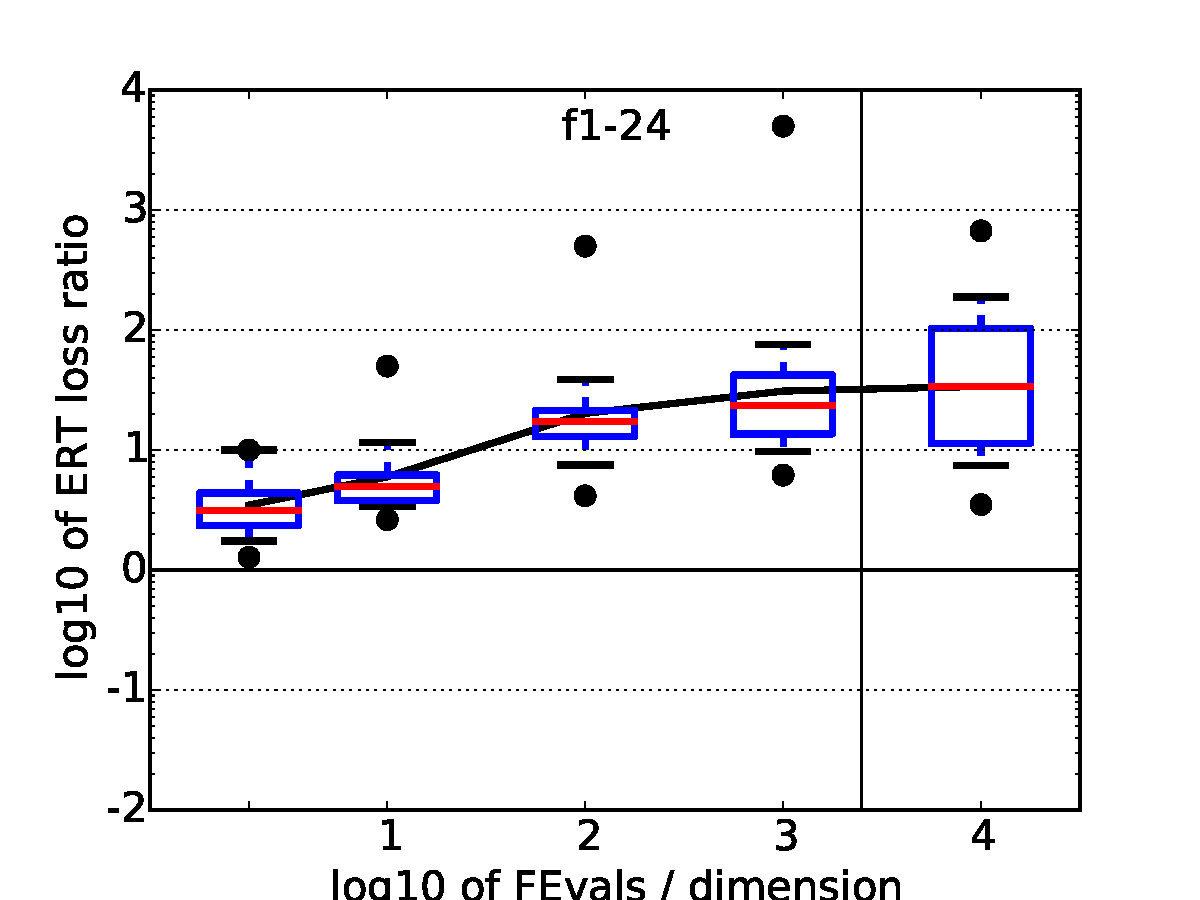
\includegraphics[width=0.24\textwidth,trim=0 0 16mm 12mm, clip]{pplogloss_05D_noiselessall} &
%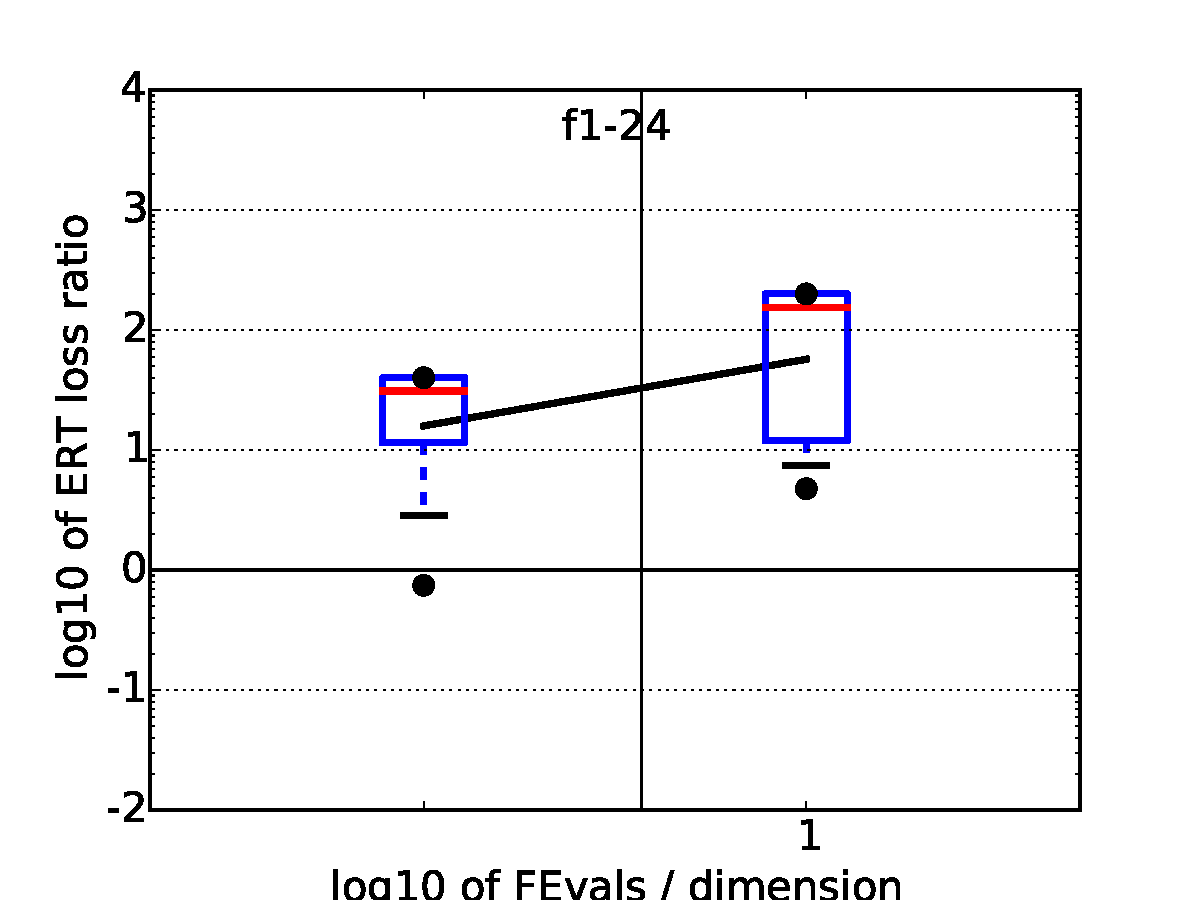
\includegraphics[width=0.24\textwidth,trim=7mm 0 9mm 12mm, clip]{pplogloss_20D_noiselessall}\\[-2ex]
\rot{separable fcts}
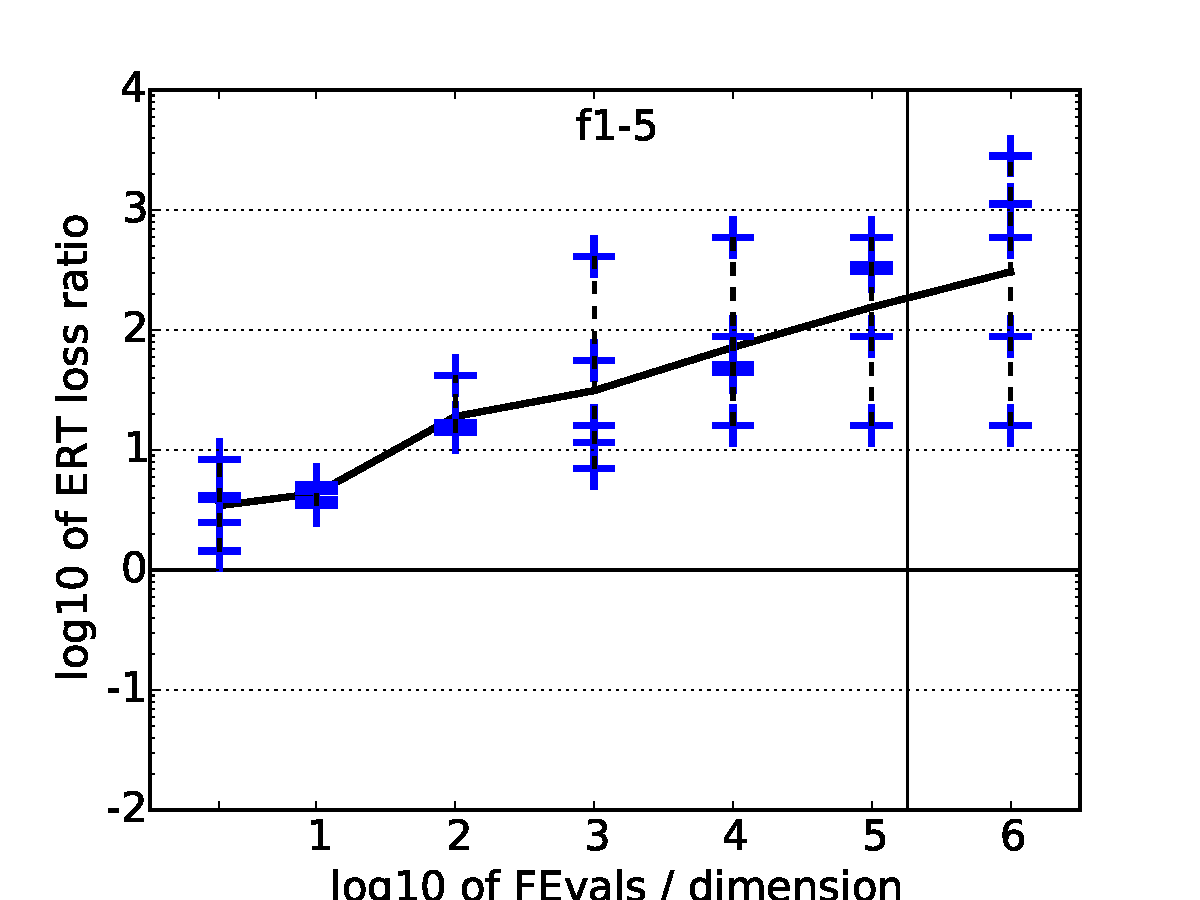
\includegraphics[width=0.35\textwidth,trim=9mm 5mm 18mm 12mm, clip]{pplogloss_05D_separ} &
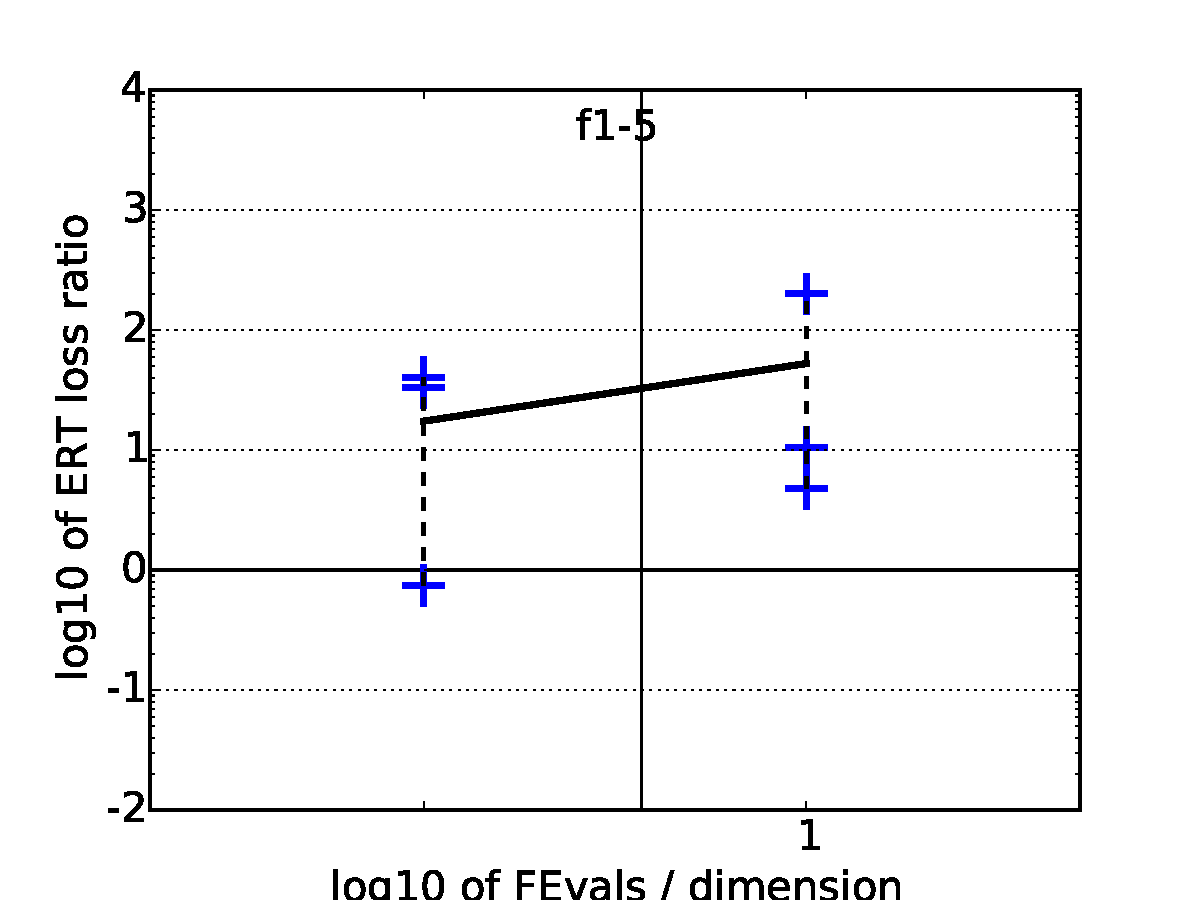
\includegraphics[width=0.35\textwidth,trim=9mm 5mm 18mm 12mm, clip]{pplogloss_20D_separ}\\[-2ex]
\rot[2]{moderate fcts}
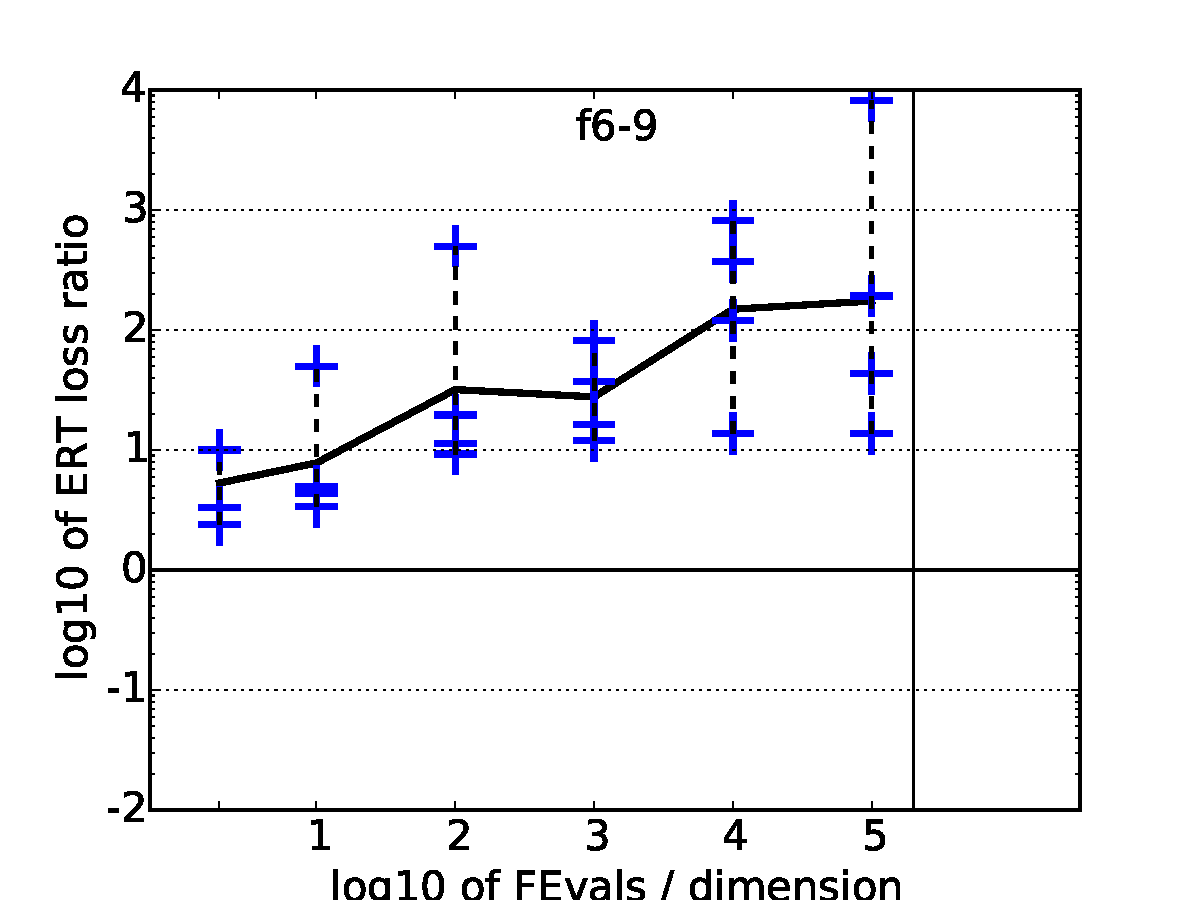
\includegraphics[width=0.35\textwidth,trim=9mm 5mm 18mm 12mm, clip]{pplogloss_05D_lcond} &
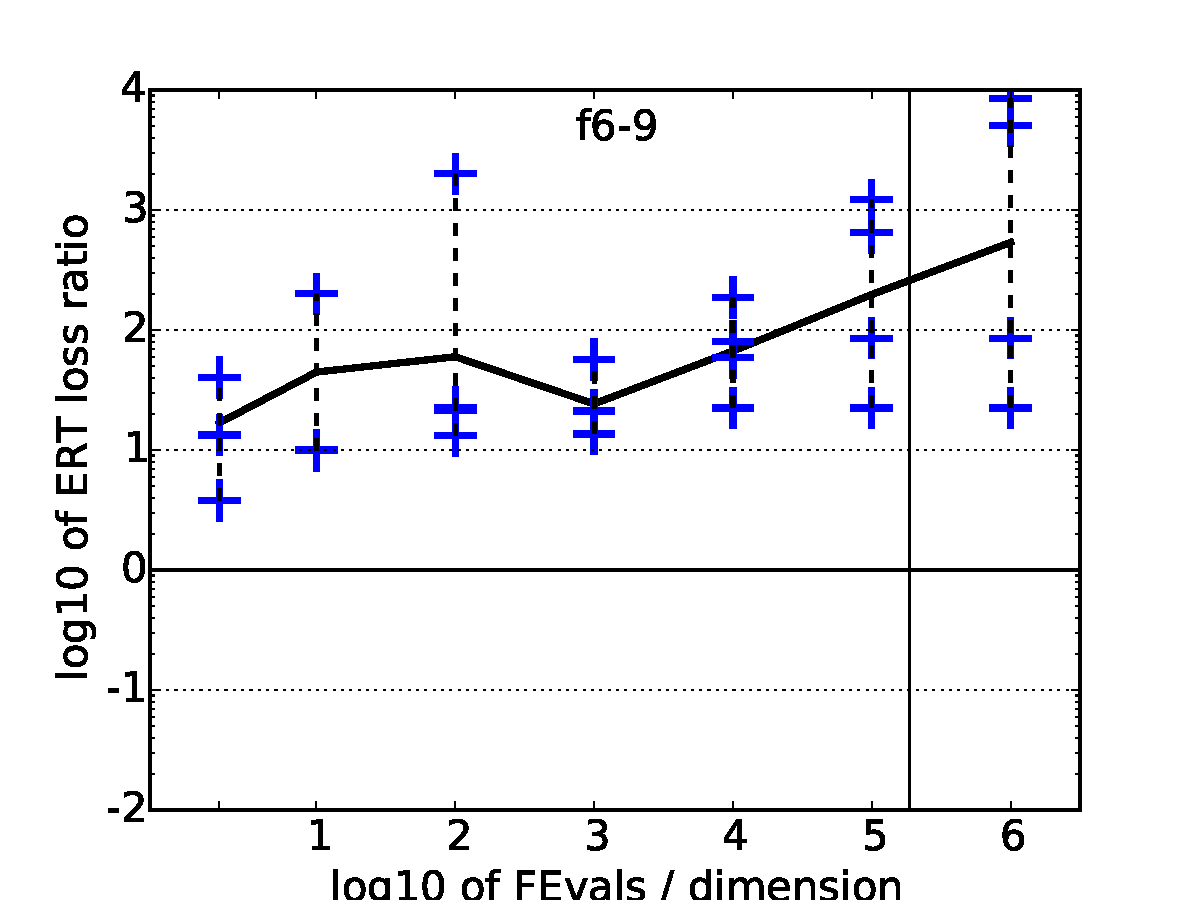
\includegraphics[width=0.35\textwidth,trim=9mm 5mm 18mm 12mm, clip]{pplogloss_20D_lcond}\\[-2ex]
\rot[1.3]{ill-conditioned fcts}
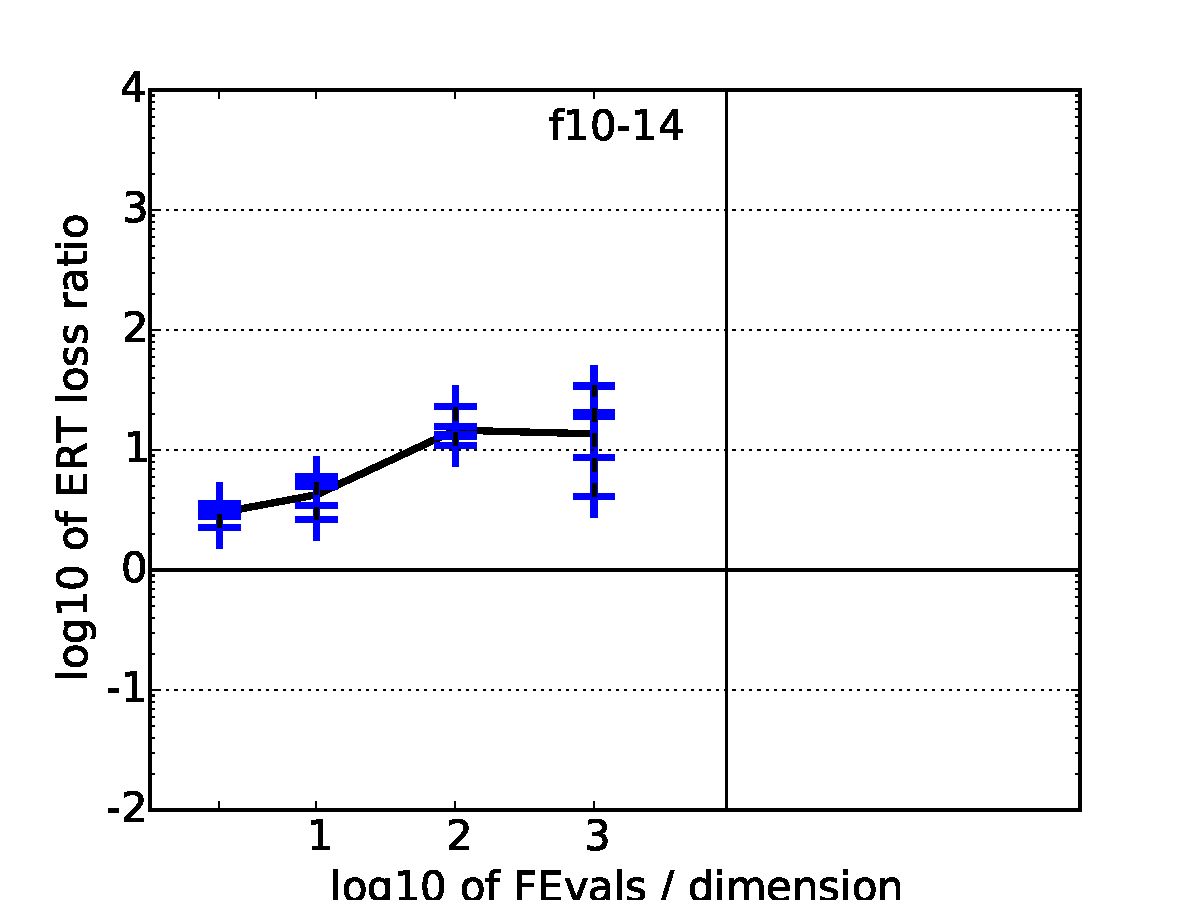
\includegraphics[width=0.35\textwidth,trim=9mm 5mm 18mm 12mm, clip]{pplogloss_05D_hcond} &
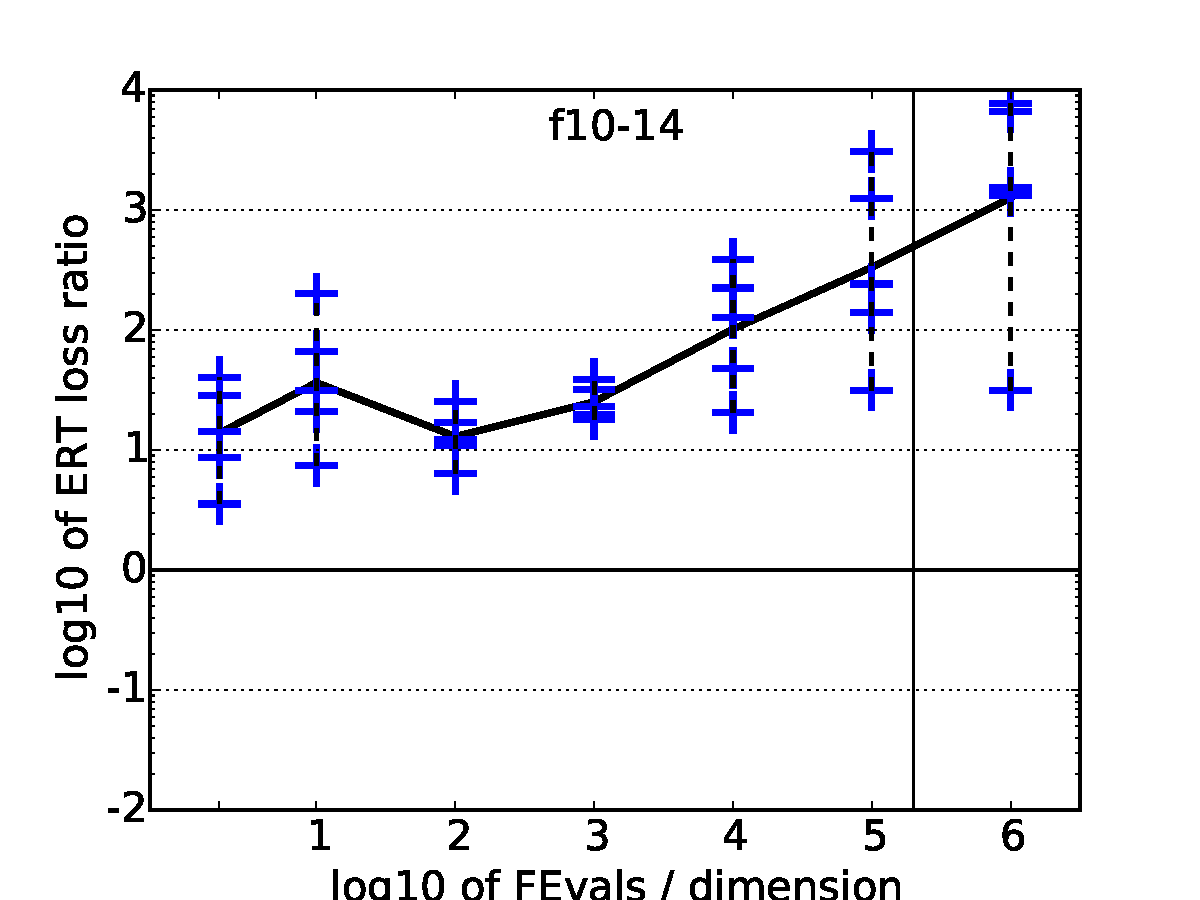
\includegraphics[width=0.35\textwidth,trim=9mm 5mm 18mm 12mm, clip]{pplogloss_20D_hcond}\\[-2ex]
\rot[1.6]{multi-modal fcts}
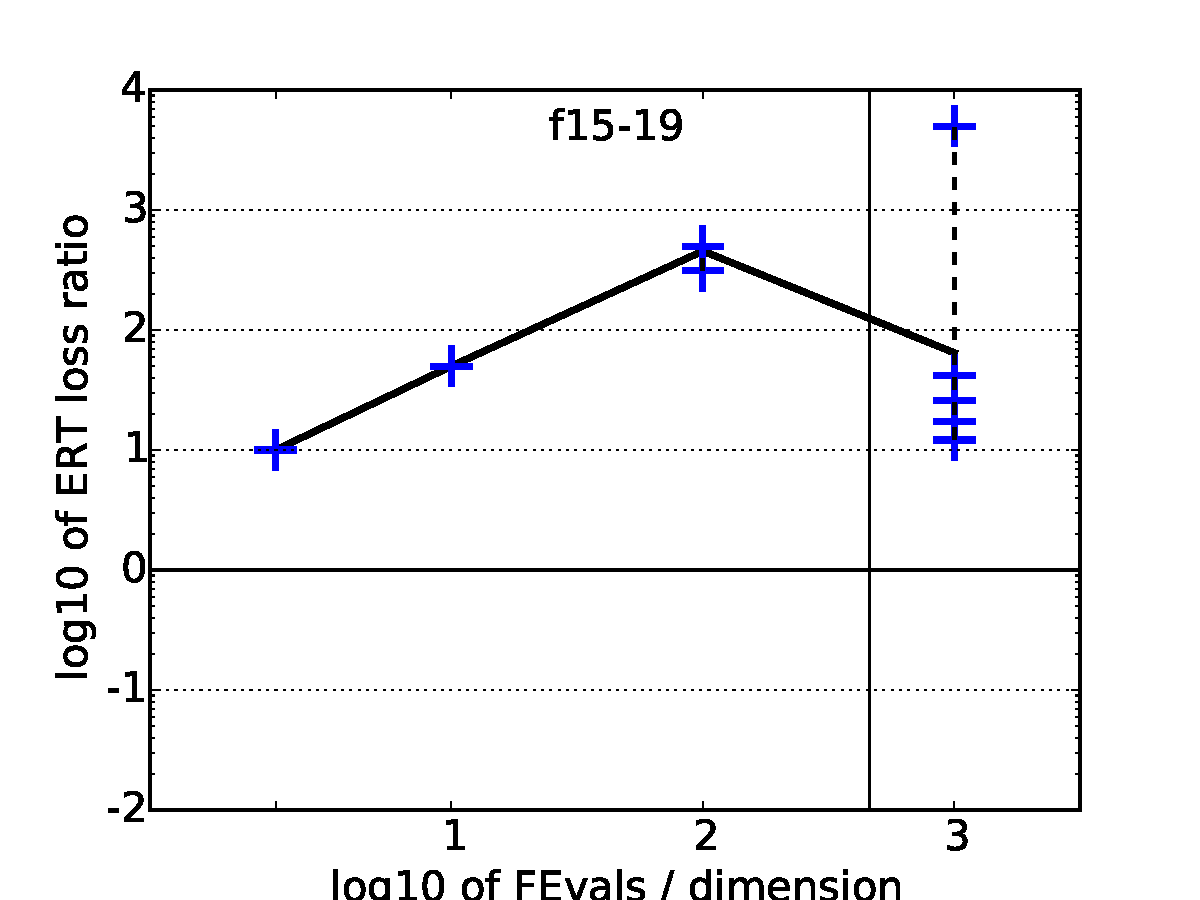
\includegraphics[width=0.35\textwidth,trim=9mm 5mm 18mm 12mm, clip]{pplogloss_05D_multi} &
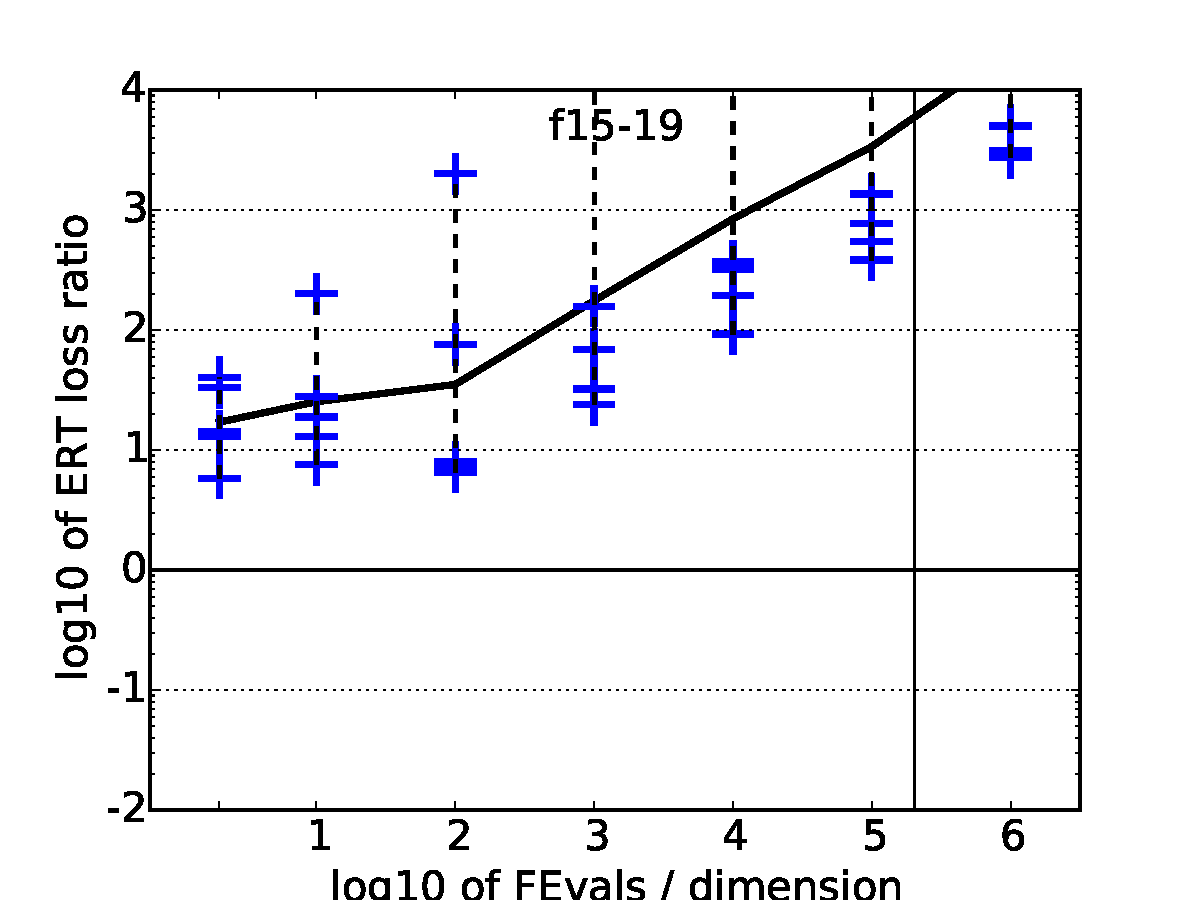
\includegraphics[width=0.35\textwidth,trim=9mm 5mm 18mm 12mm, clip]{pplogloss_20D_multi}\\[-2ex]
\rot[1.0]{weak structure fcts}
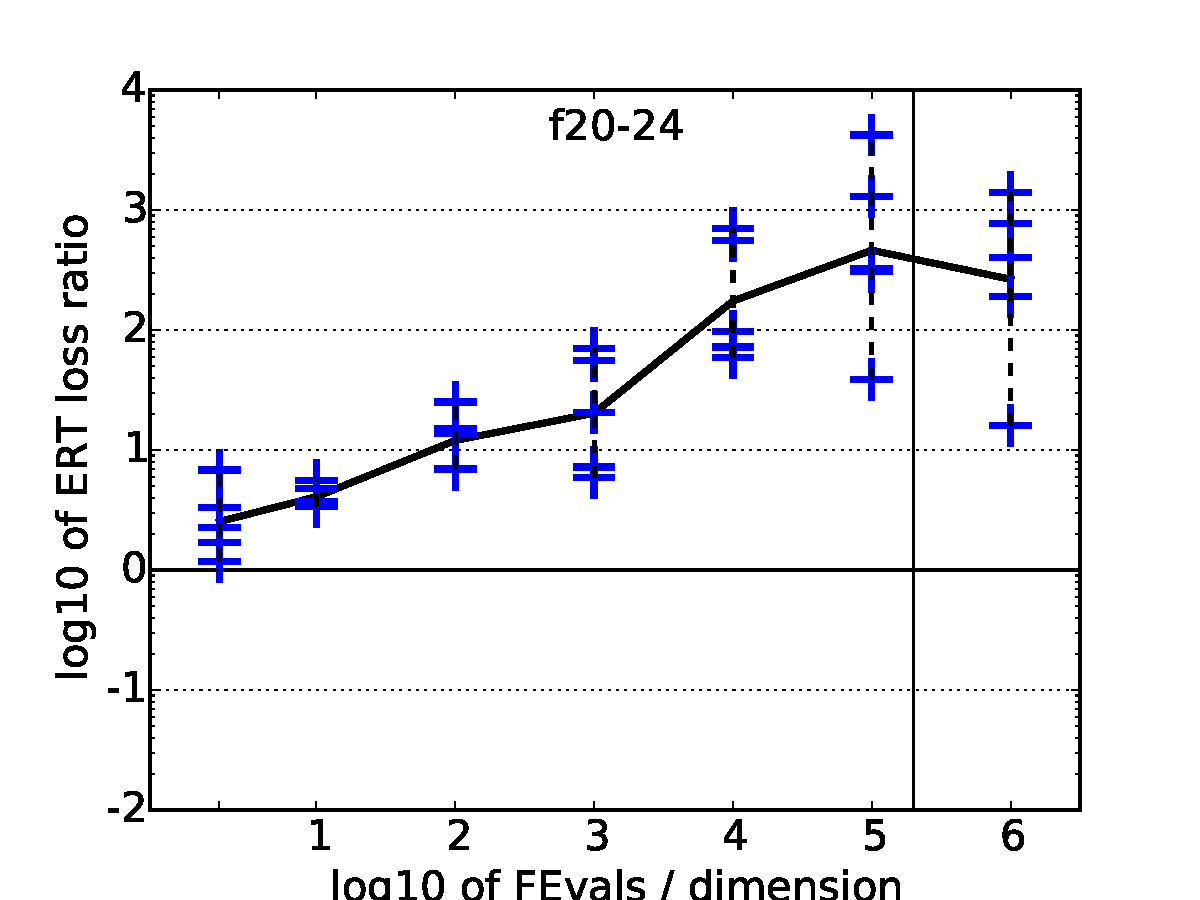
\includegraphics[width=0.35\textwidth,trim=9mm 0mm 18mm 12mm, clip]{pplogloss_05D_mult2} &
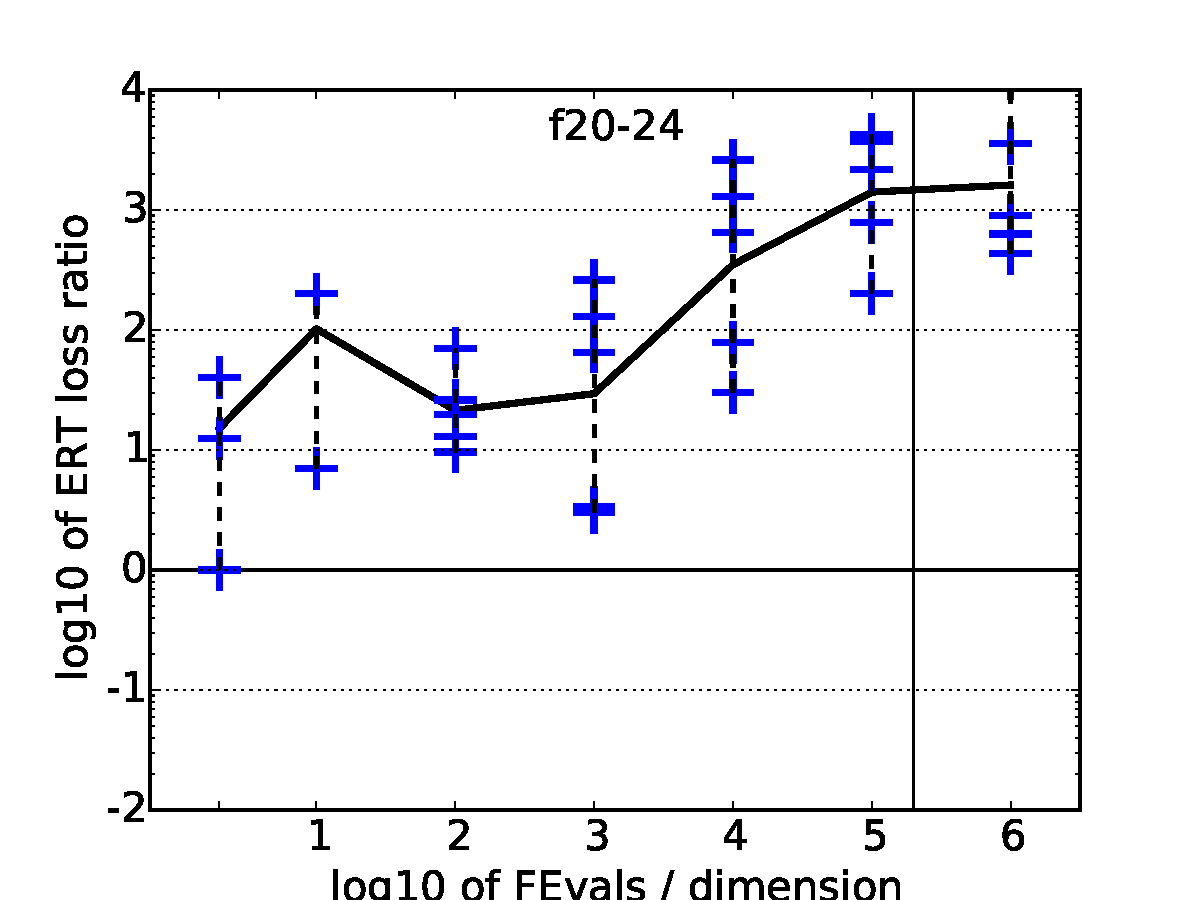
\includegraphics[width=0.35\textwidth,trim=9mm 0mm 18mm 12mm, clip]{pplogloss_20D_mult2}
\vspace*{-1ex}
\end{tabular}
\caption{\label{fig:ERTloglossb\algfolder}\ERT\ loss ratio versus given budget
$\FEvals$ divided by dimension in log-log display. Crosses give
the single values on the indicated functions, the line is the geometric mean.
The vertical line gives the maximal number of function evaluations in the
respective function subgroup.}
\end{figure}
%%%%%%%%%%%%%%%%%%%%%%%%%%%%%%%%%%%%%%%%%%%%%%%%%%%%%%%%%%%%%%%%%%%%%%%%%%%%%%%
%%%%%%%%%%%%%%%%%%%%%%%%%%%%%%%%%%%%%%%%%%%%%%%%%%%%%%%%%%%%%%%%%%%%%%%%%%%%%%%
\begin{figure}[htbp!]
\begin{tabular}{@{}c@{}c@{}c@{}c@{}}
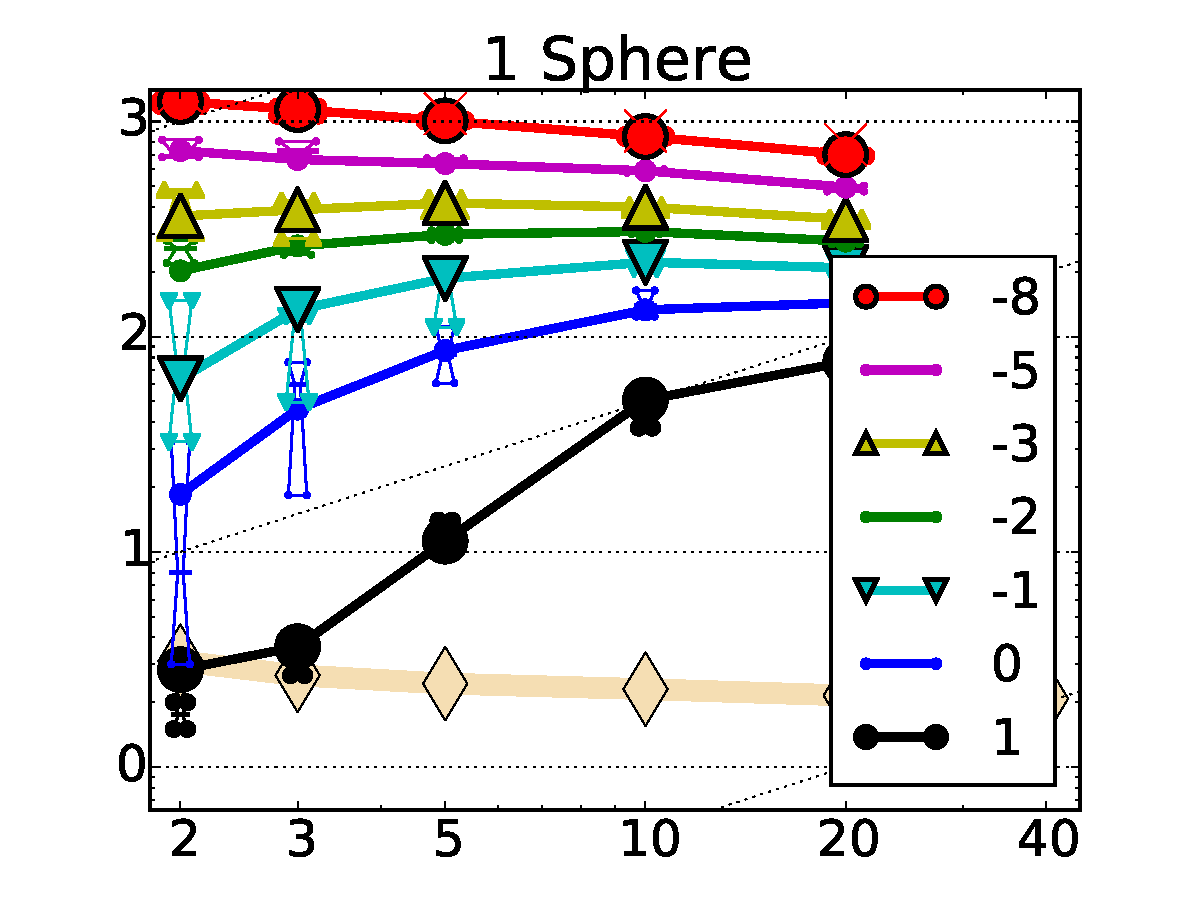
\includegraphics[width=0.25\textwidth, trim=20mm 7mm 15mm 3mm, clip]{ppfigdim_f001}&
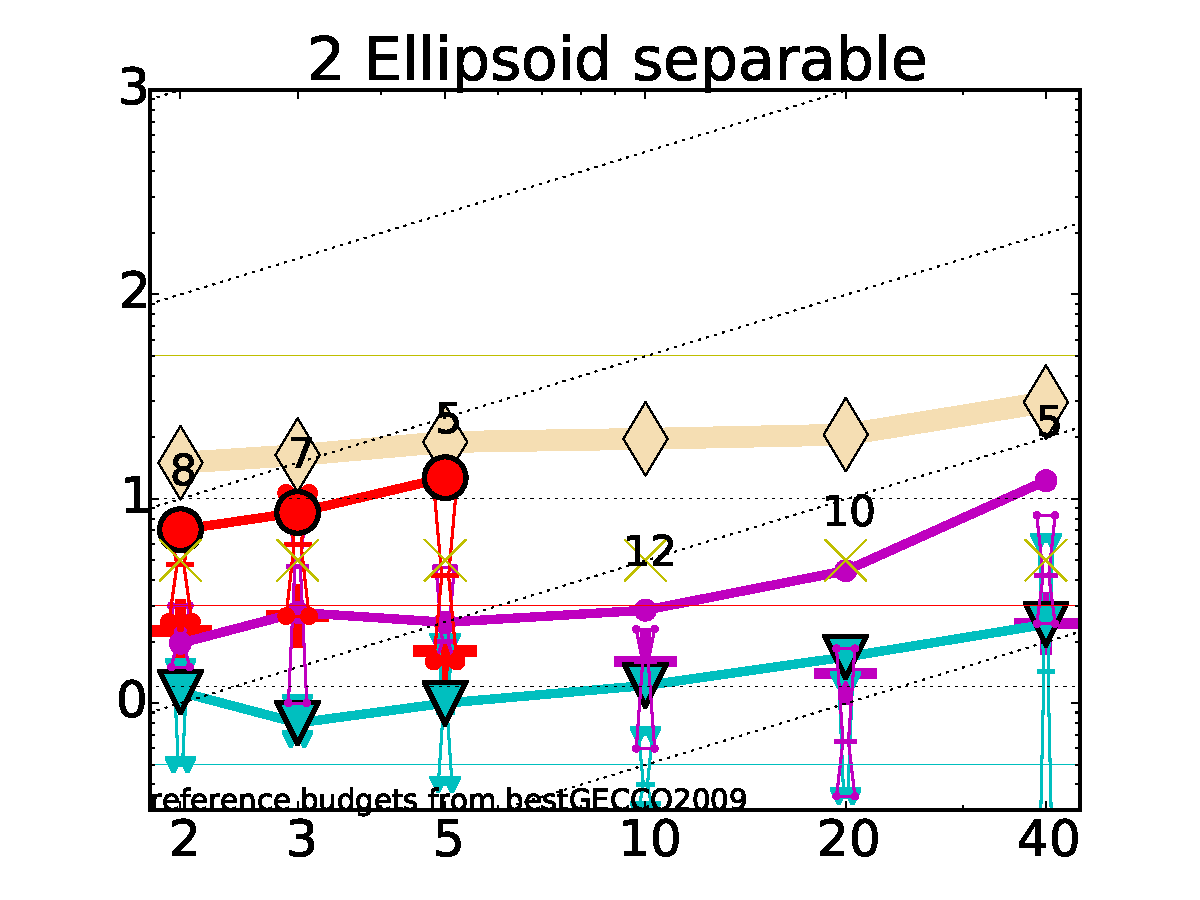
\includegraphics[width=0.25\textwidth, trim=20mm 7mm 15mm 3mm, clip]{ppfigdim_f002}&
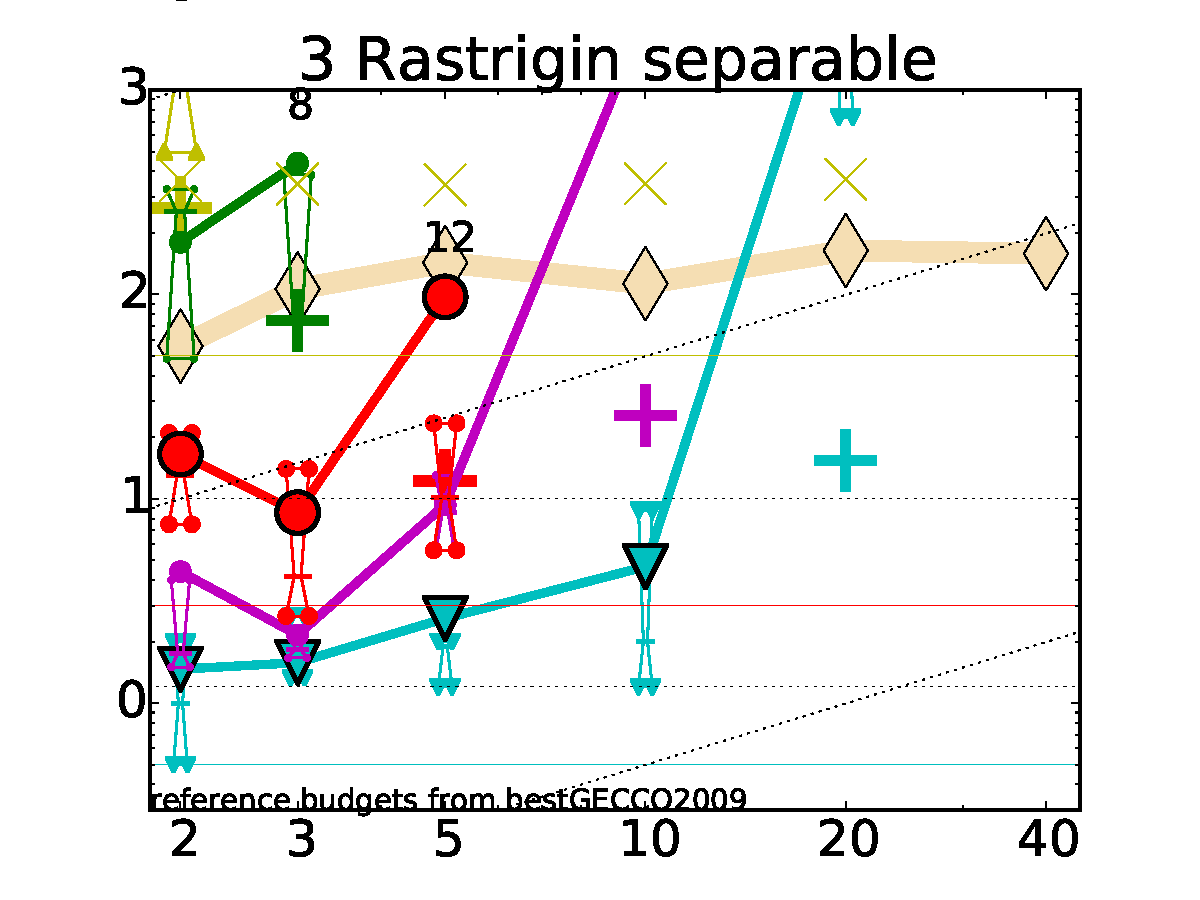
\includegraphics[width=0.25\textwidth, trim=20mm 7mm 15mm 3mm, clip]{ppfigdim_f003}&
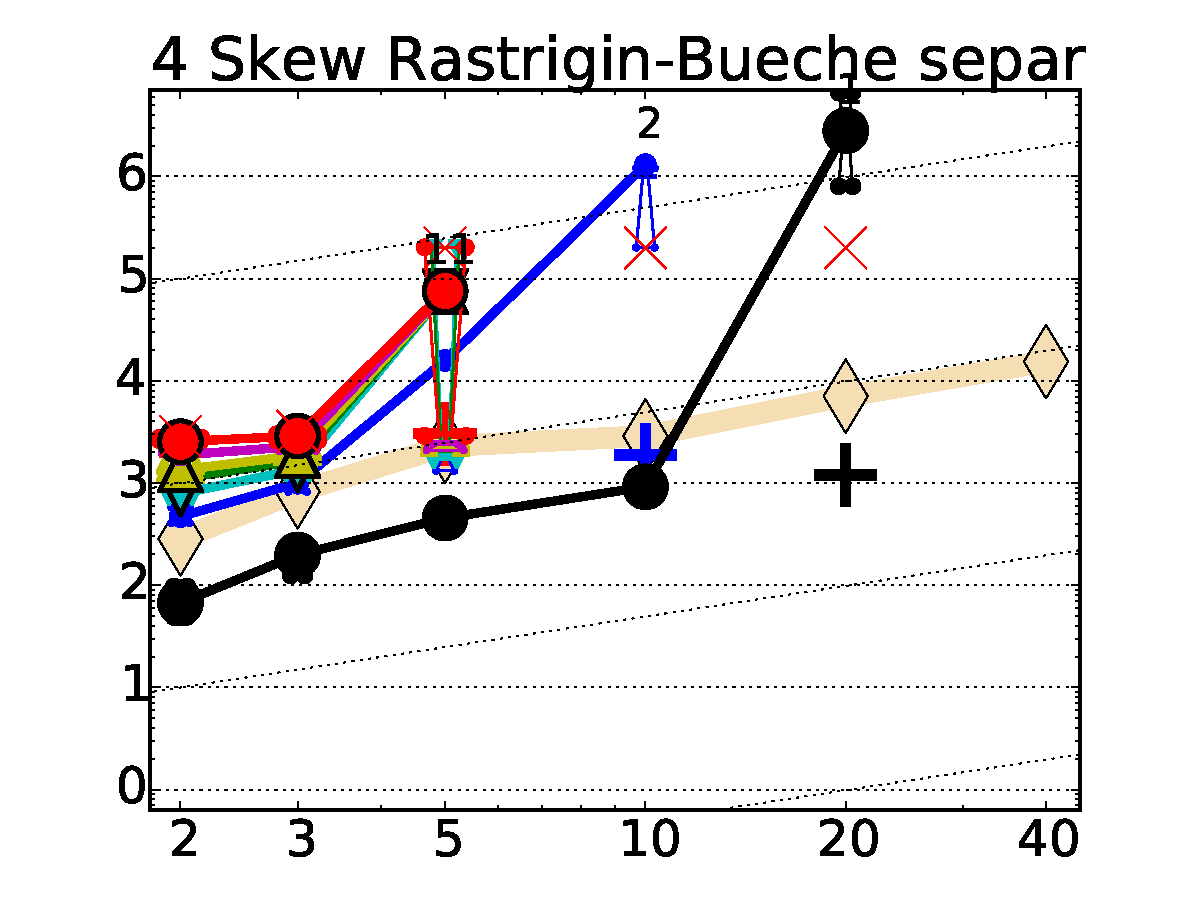
\includegraphics[width=0.25\textwidth, trim=20mm 7mm 15mm 3mm, clip]{ppfigdim_f004}\\
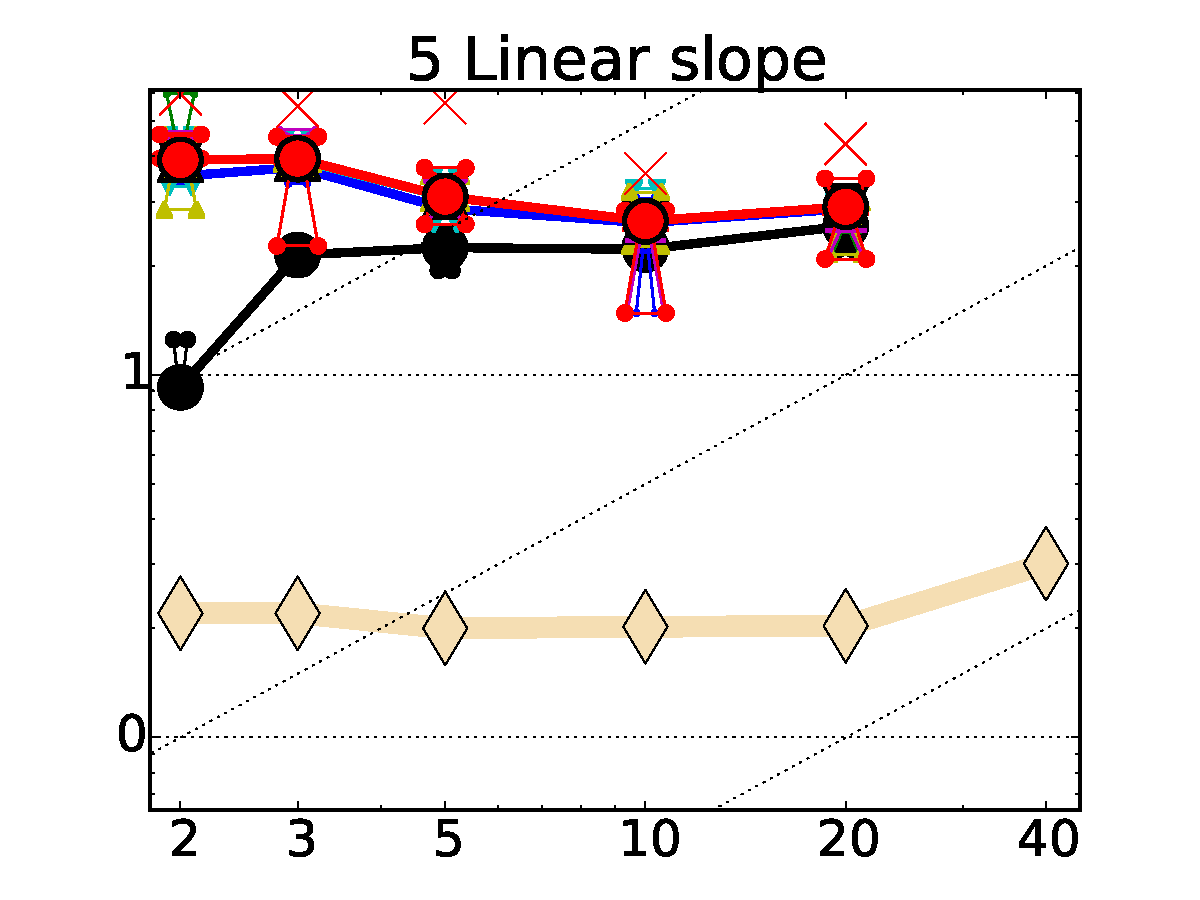
\includegraphics[width=0.25\textwidth, trim=20mm 7mm 15mm 3mm, clip]{ppfigdim_f005}&
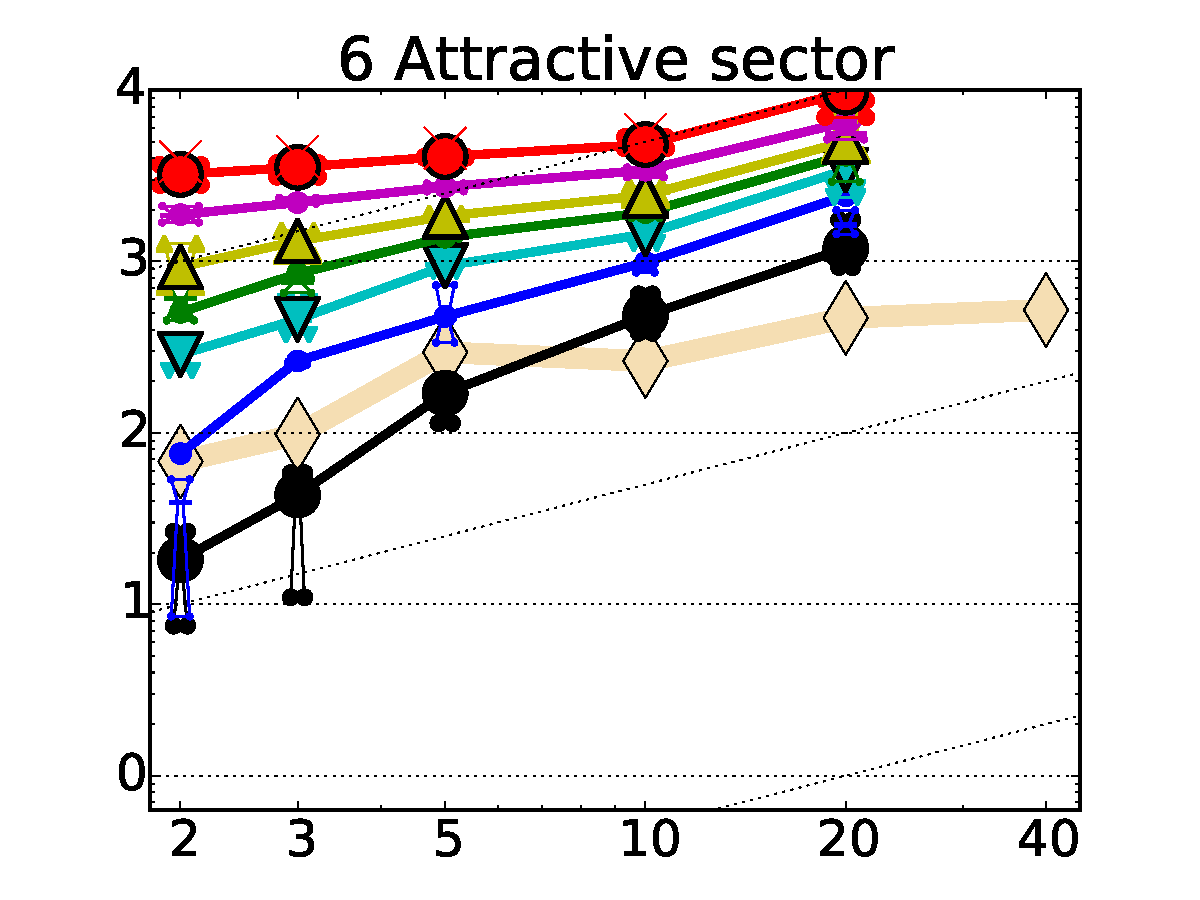
\includegraphics[width=0.25\textwidth, trim=20mm 7mm 15mm 3mm, clip]{ppfigdim_f006}&
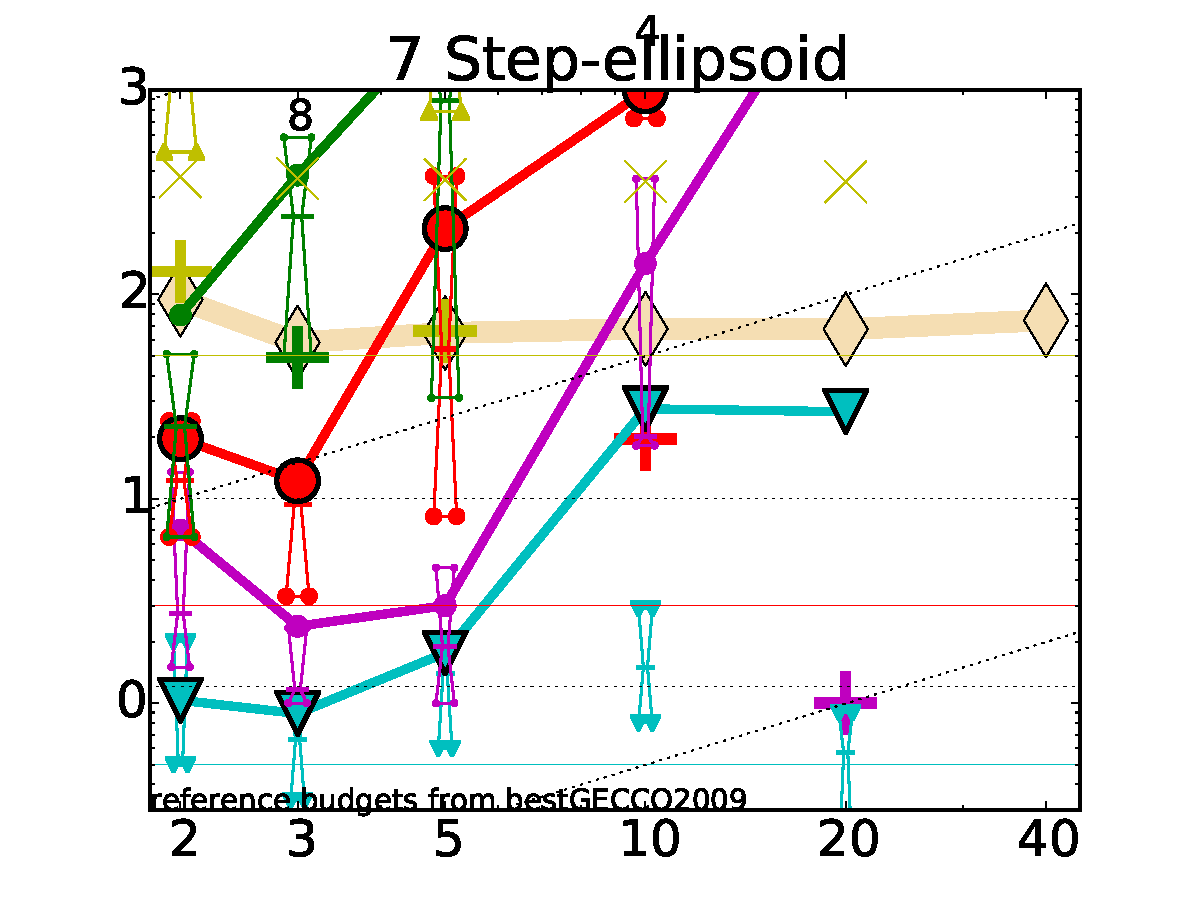
\includegraphics[width=0.25\textwidth, trim=20mm 7mm 15mm 3mm, clip]{ppfigdim_f007}&
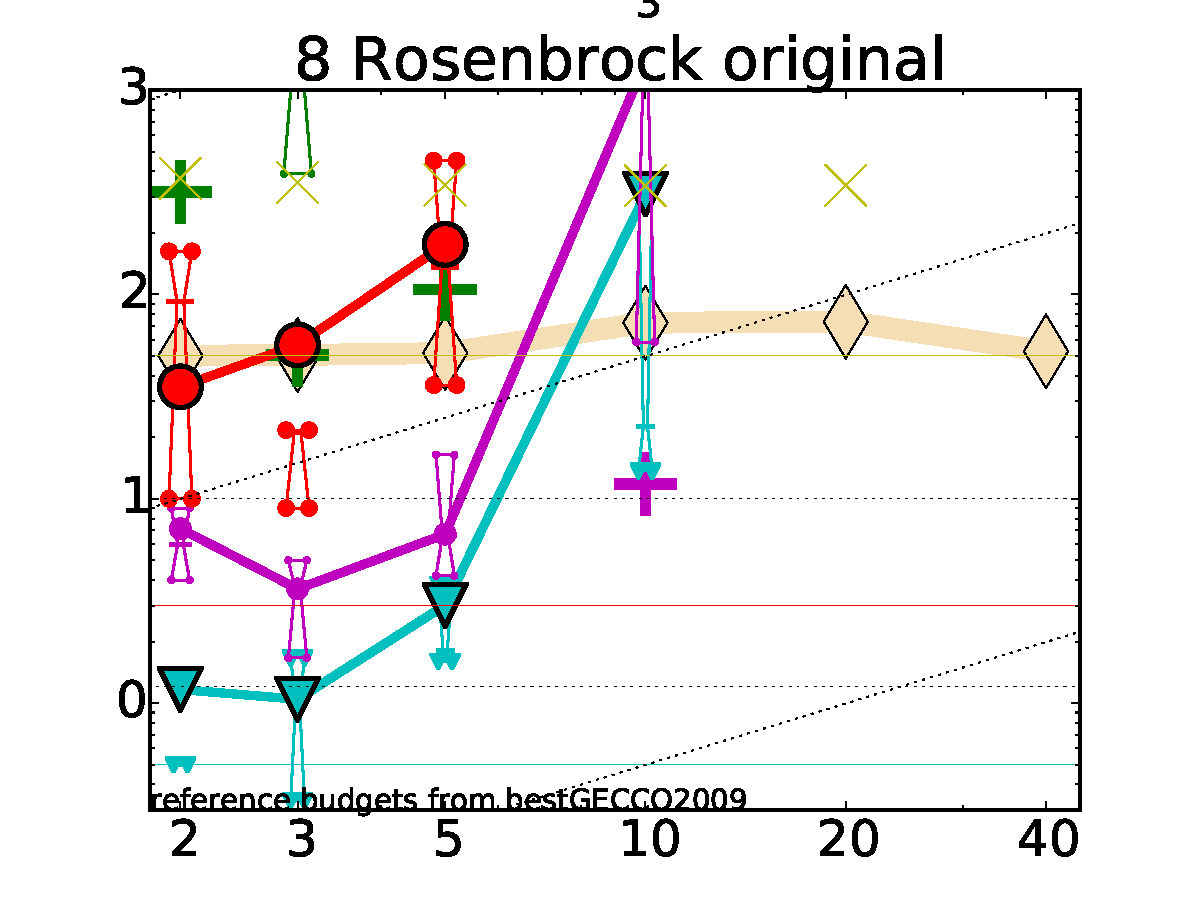
\includegraphics[width=0.25\textwidth, trim=20mm 7mm 15mm 3mm, clip]{ppfigdim_f008}\\
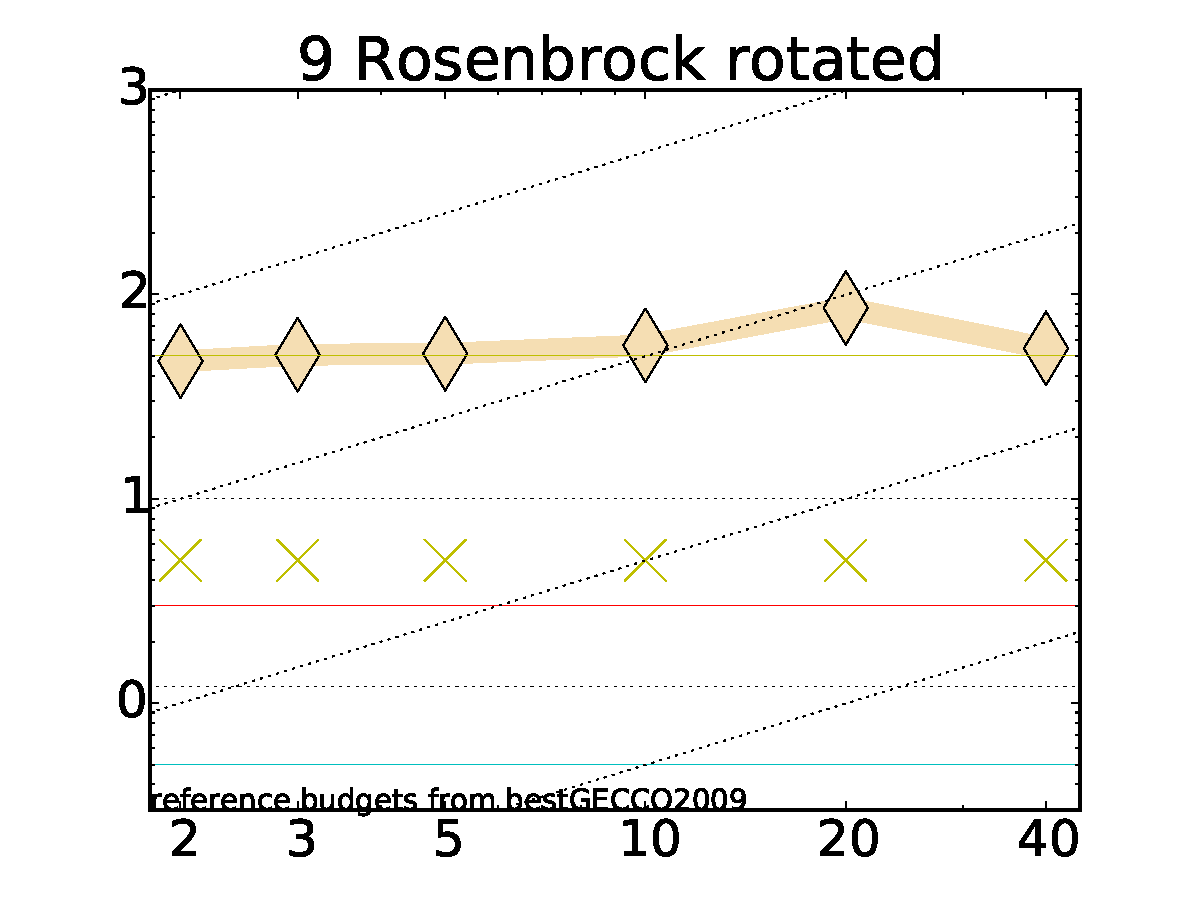
\includegraphics[width=0.25\textwidth, trim=20mm 7mm 15mm 3mm, clip]{ppfigdim_f009}&
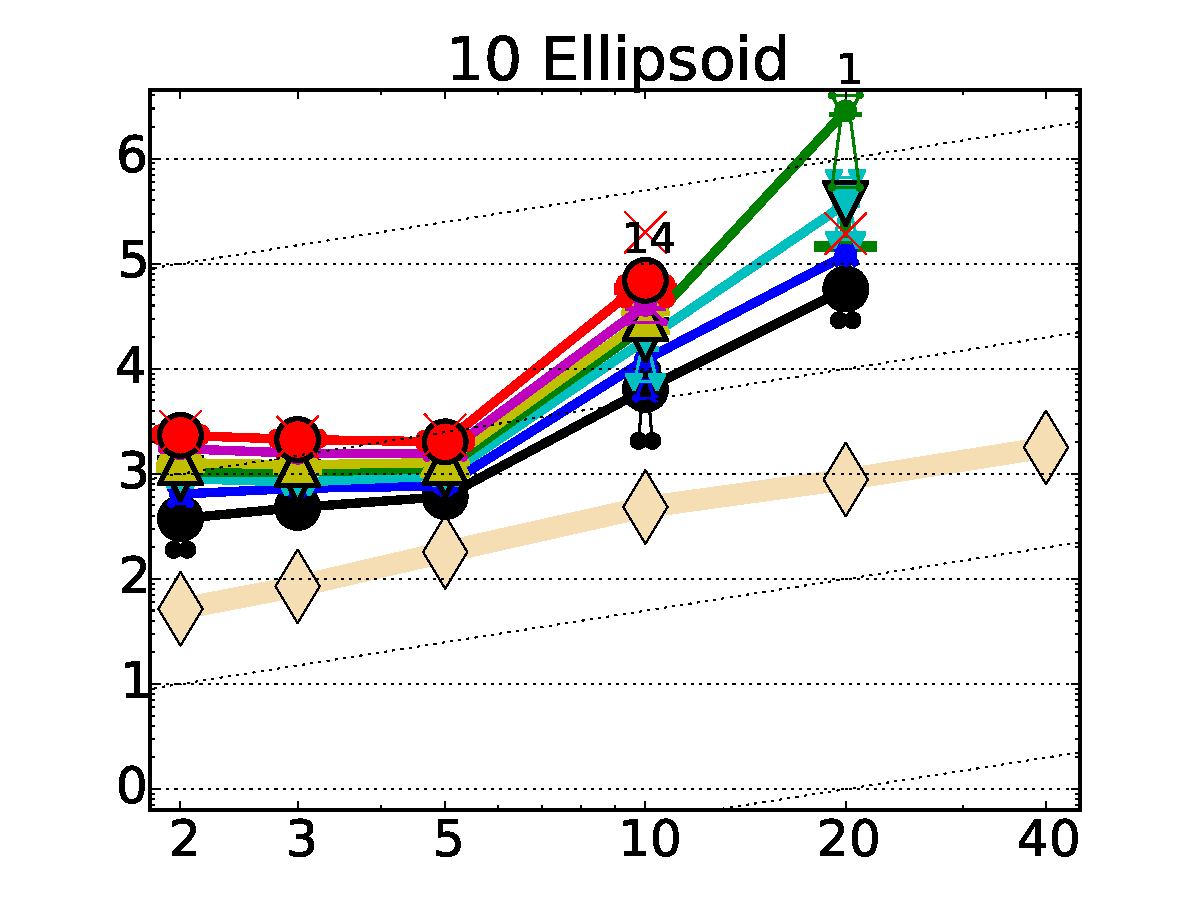
\includegraphics[width=0.25\textwidth, trim=20mm 7mm 15mm 3mm, clip]{ppfigdim_f010}&
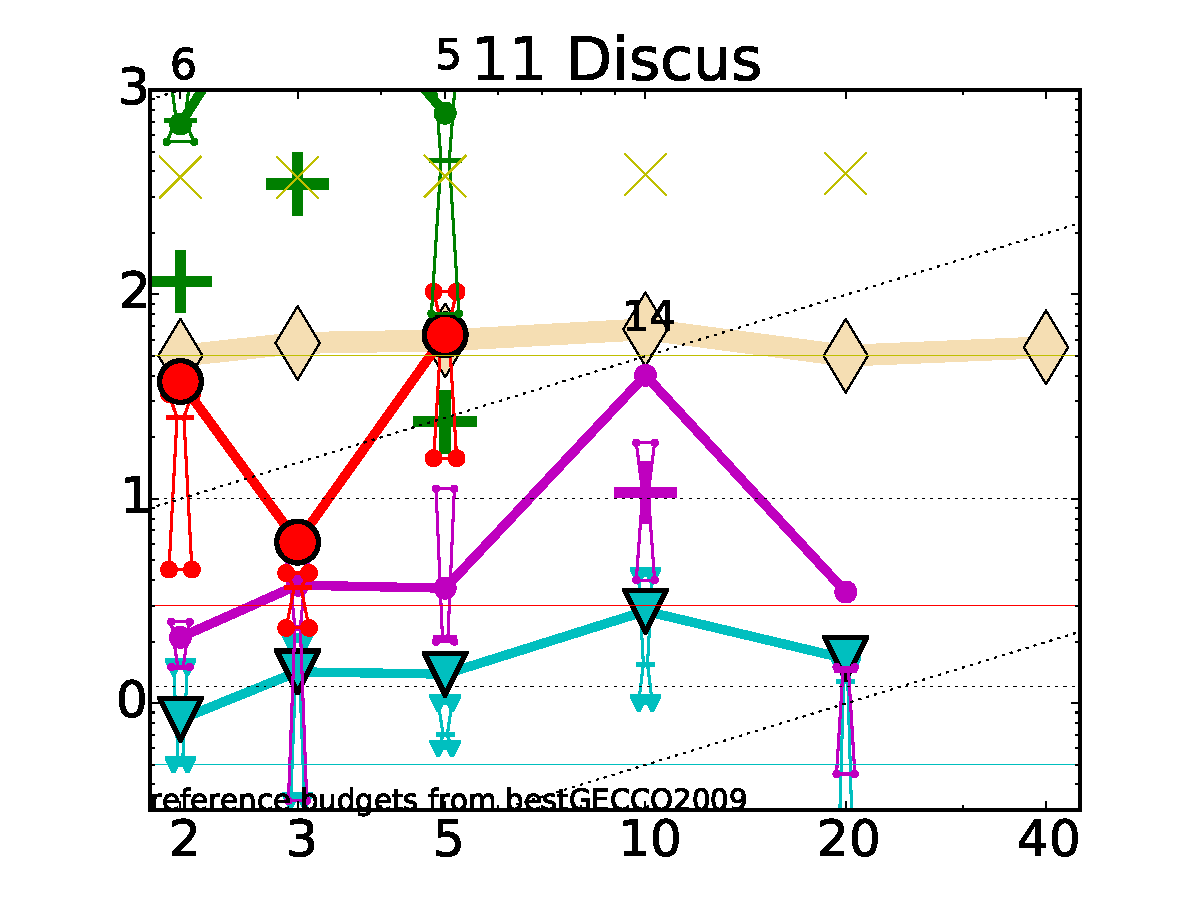
\includegraphics[width=0.25\textwidth, trim=20mm 7mm 15mm 3mm, clip]{ppfigdim_f011}&
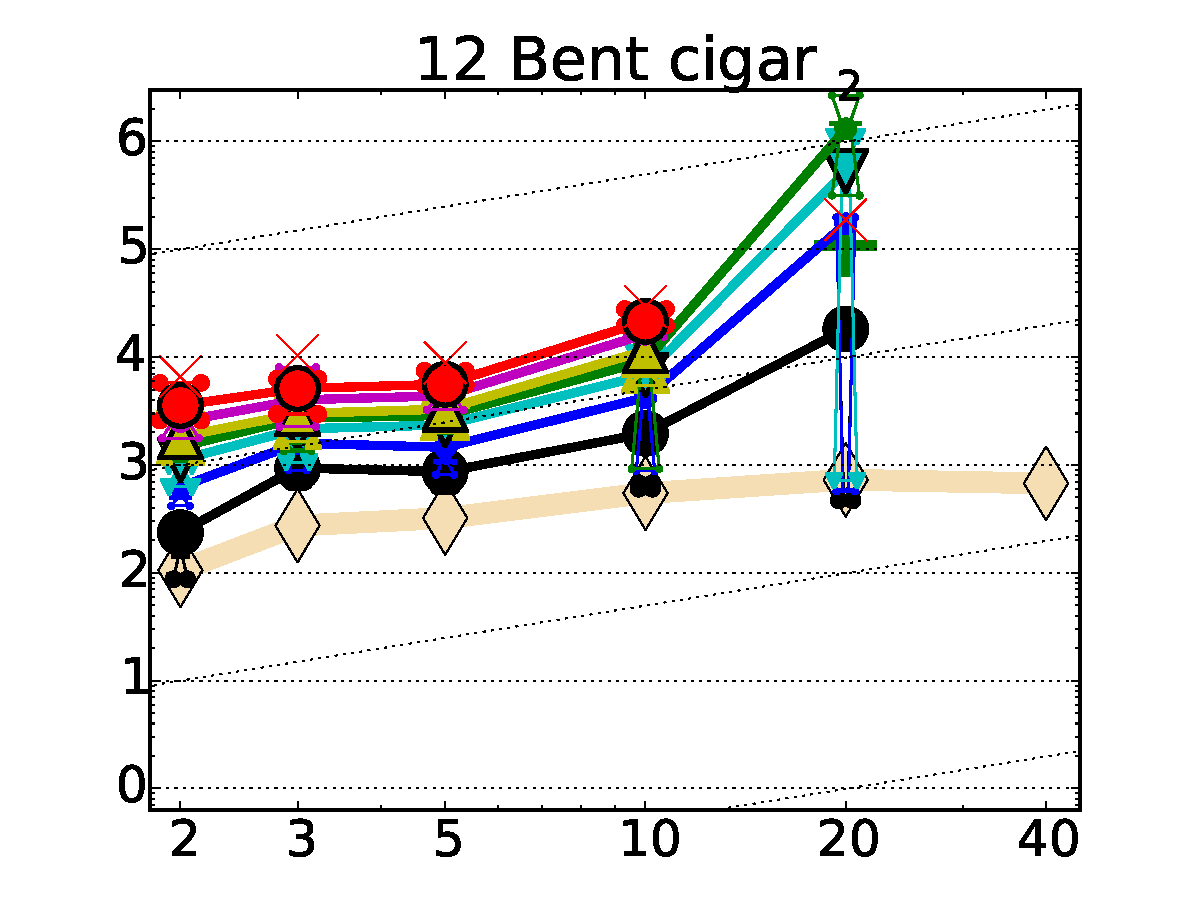
\includegraphics[width=0.25\textwidth, trim=20mm 7mm 15mm 3mm, clip]{ppfigdim_f012}\\
\includegraphics[width=0.25\textwidth, trim=20mm 7mm 15mm 3mm, clip]{ppfigdim_f013}&
\includegraphics[width=0.25\textwidth, trim=20mm 7mm 15mm 3mm, clip]{ppfigdim_f014}&
\includegraphics[width=0.25\textwidth, trim=20mm 7mm 15mm 3mm, clip]{ppfigdim_f015}&
\includegraphics[width=0.25\textwidth, trim=20mm 7mm 15mm 3mm, clip]{ppfigdim_f016}\\
\includegraphics[width=0.25\textwidth, trim=20mm 7mm 15mm 3mm, clip]{ppfigdim_f017}&
\includegraphics[width=0.25\textwidth, trim=20mm 7mm 15mm 3mm, clip]{ppfigdim_f018}&
\includegraphics[width=0.25\textwidth, trim=20mm 7mm 15mm 3mm, clip]{ppfigdim_f019}&
\includegraphics[width=0.25\textwidth, trim=20mm 7mm 15mm 3mm, clip]{ppfigdim_f020}\\
\includegraphics[width=0.25\textwidth, trim=20mm 7mm 15mm 3mm, clip]{ppfigdim_f021}&
\includegraphics[width=0.25\textwidth, trim=20mm 7mm 15mm 3mm, clip]{ppfigdim_f022}&
\includegraphics[width=0.25\textwidth, trim=20mm 7mm 15mm 3mm, clip]{ppfigdim_f023}&
\includegraphics[width=0.25\textwidth, trim=20mm 7mm 15mm 3mm, clip]{ppfigdim_f024}
\end{tabular}
\vspace*{-1ex}
\caption{\label{fig:ERTgraphs\algfolder}
\bbobppfigdimlegend{$f_1$ and $f_{24}$}
%Expected running time (\ERT) divided by
%dimension versus dimension in log-log presentation. Shown are different target
%values $\fopt+\Df$, where 
%% $\Df = 10, 1, 10^{-1}, 10^{-2}, 10^{-3}, 10^{-5}, 10^{-8}$
%$\Df = 10^{\{+1, 0, -1, -2, -3, -5, -8\}}$ and the exponent is given in the
%legend of $f_1$ and $f_{24}$. Plus symbols ($+$) show the median number of
%$f$-evaluations for the best reached target value. Crosses ($\times$) indicate
%the total number of $f$-evaluations ($\nbFEs(-\infty)$) divided by the number
%of trials. Numbers above \ERT-symbols indicate the number of successful trials.
%Y-axis annotations are decimal logarithms.
%%The thick light line with diamond
%%markers shows the single best results from BBOB 2009 for
%%$\Df=10^{-8}$.
}
\end{figure}
%%%%%%%%%%%%%%%%%%%%%%%%%%%%%%%%%%%%%%%%%%%%%%%%%%%%%%%%%%%%%%%%%%%%%%%%%%%%%%%
%%%%%%%%%%%%%%%%%%%%%%%%%%%%%%%%%%%%%%%%%%%%%%%%%%%%%%%%%%%%%%%%%%%%%%%%%%%%%%%
\begin{table}[htbp!]
\centering
\footnotesize
\input{\bbobdatapath\algfolder pptable_05D_noiselessall}
\caption{\label{tab:ERT05D\algfolder} \bbobpptablecaption{} Results of \algname\ in 5-D.}
\end{table}
%%%%%%%%%%%%%%%%%%%%%%%%%%%%%%%%%%%%%%%%%%%%%%%%%%%%%%%%%%%%%%%%%%%%%%%%%%%%%%%
%%%%%%%%%%%%%%%%%%%%%%%%%%%%%%%%%%%%%%%%%%%%%%%%%%%%%%%%%%%%%%%%%%%%%%%%%%%%%%%
\begin{table}[htbp!]
\centering
\footnotesize
\input{\bbobdatapath\algfolder pptable_20D_noiselessall}
\caption{\label{tab:ERT20D\algfolder} \bbobpptablecaption{} Results of \algname\ in 20-D.}
\end{table}
%%%%%%%%%%%%%%%%%%%%%%%%%%%%%%%%%%%%%%%%%%%%%%%%%%%%%%%%%%%%%%%%%%%%%%%%%%%%%%%
%%%%%%%%%%%%%%%%%%%%%%%%%%%%%%%%%%%%%%%%%%%%%%%%%%%%%%%%%%%%%%%%%%%%%%%%%%%%%%%
% The following two commands are all you need in the
% initial runs of your .tex file to
% produce the bibliography for the citations in your paper.
\bibliographystyle{abbrv}
\bibliography{bbob} % bbob.bib is the name of the bib file in this case
% You must have a proper ".bib" file
%  and remember to run:
% latex bibtex latex latex
% to resolve all references
\end{document}

